\documentclass[11pt]{article}

\usepackage[margin=1in]{geometry}
\usepackage{amsmath,amssymb}
\usepackage{graphicx}
\usepackage{booktabs}
\usepackage{xcolor}
\usepackage{multirow}
\usepackage[font=small,labelfont=bf]{caption}
\usepackage[hidelinks]{hyperref}
\usepackage{siunitx}
\usepackage{array}

\sisetup{detect-all}

\newcommand{\re}{\mathrm{Re}}

\title{\large Supplementary material:\\ Physics-informed identification and independent validation of conditional modal collapse in active control of lid-driven cavity flow}

\author{Ahmed Beniaiche, Abderrahim Larabi, Abderrahim Dourari, and Mbarek Belkadi}

\date{}

\begin{document}

\maketitle

This document collects the supplementary figures and tables that support the main text. Section and figure references that contain a number correspond to the main text.

\section{Network architecture sweep}\label{ssec:archtable}

Table~S1 complements the architecture column of the architecture-robustness table of the main text with the realized energies, parameter counts, and temporal fractions of the small and large networks. All runs are at $\re=500$ with the Fourier basis, three independent seeds per architecture, and $E^*=0.25$. The seed of the baseline network that coincides with the intermediate branch of the main-text seed study is excluded from the reported range.

\begin{table}[h]
\centering
\caption{Network architecture sweep at $\re=500$, Fourier basis, three seeds per architecture. $n_{\mathrm{par}}$: number of trainable parameters; $E_r$: realized-energy range; $f_2$: second-mode fraction range; $f_t$: temporal fraction range.}
\label{tab:s1}
\begin{tabular}{lcccc}
\toprule
Architecture (head) & $n_{\mathrm{par}}$ & $E_r$ & $f_2$ (\%) & $f_t$ (\%) \\
\midrule
Small $[64,64,32]$        & 8774    & 0.244--0.276 & 90.3--93.6 & $<$2 \\
Baseline $[128,128,96,64]$ & 44824   & 0.240--0.267 & 89.2--91.1$^{*}$ & $\lesssim$5 \\
Large $[256,256,128,96]$  & 139624  & 0.252--0.257 & 86.7--92.2 & $\lesssim$5 \\
\bottomrule
\end{tabular}
\end{table}

$^{*}$Excluding the seed associated with the intermediate branch of the main-text seed study.

The architecture sweep shows that the Mode-2 branch can be recovered across the three tested network capacities. Both the smallest and the largest networks considered converge to a second-mode-dominant state with $f_2$ in the high-80s to low-90s percentile, consistent with the baseline network used throughout the main text. The parameter count varies by more than an order of magnitude across the three architectures.

\section{Velocity and dissipation fields}

Figures~S1 and~S2 show the velocity magnitude and the viscous dissipation fields of the controlled flow at $\re=100$, $500$, and $1000$, for the Fourier branch recovered in the main text, as realized by the independent LBM solver. The central circulation produced by the dominant second spatial mode and the corresponding dissipation concentration are apparent.

\begin{figure}[h]
\centering
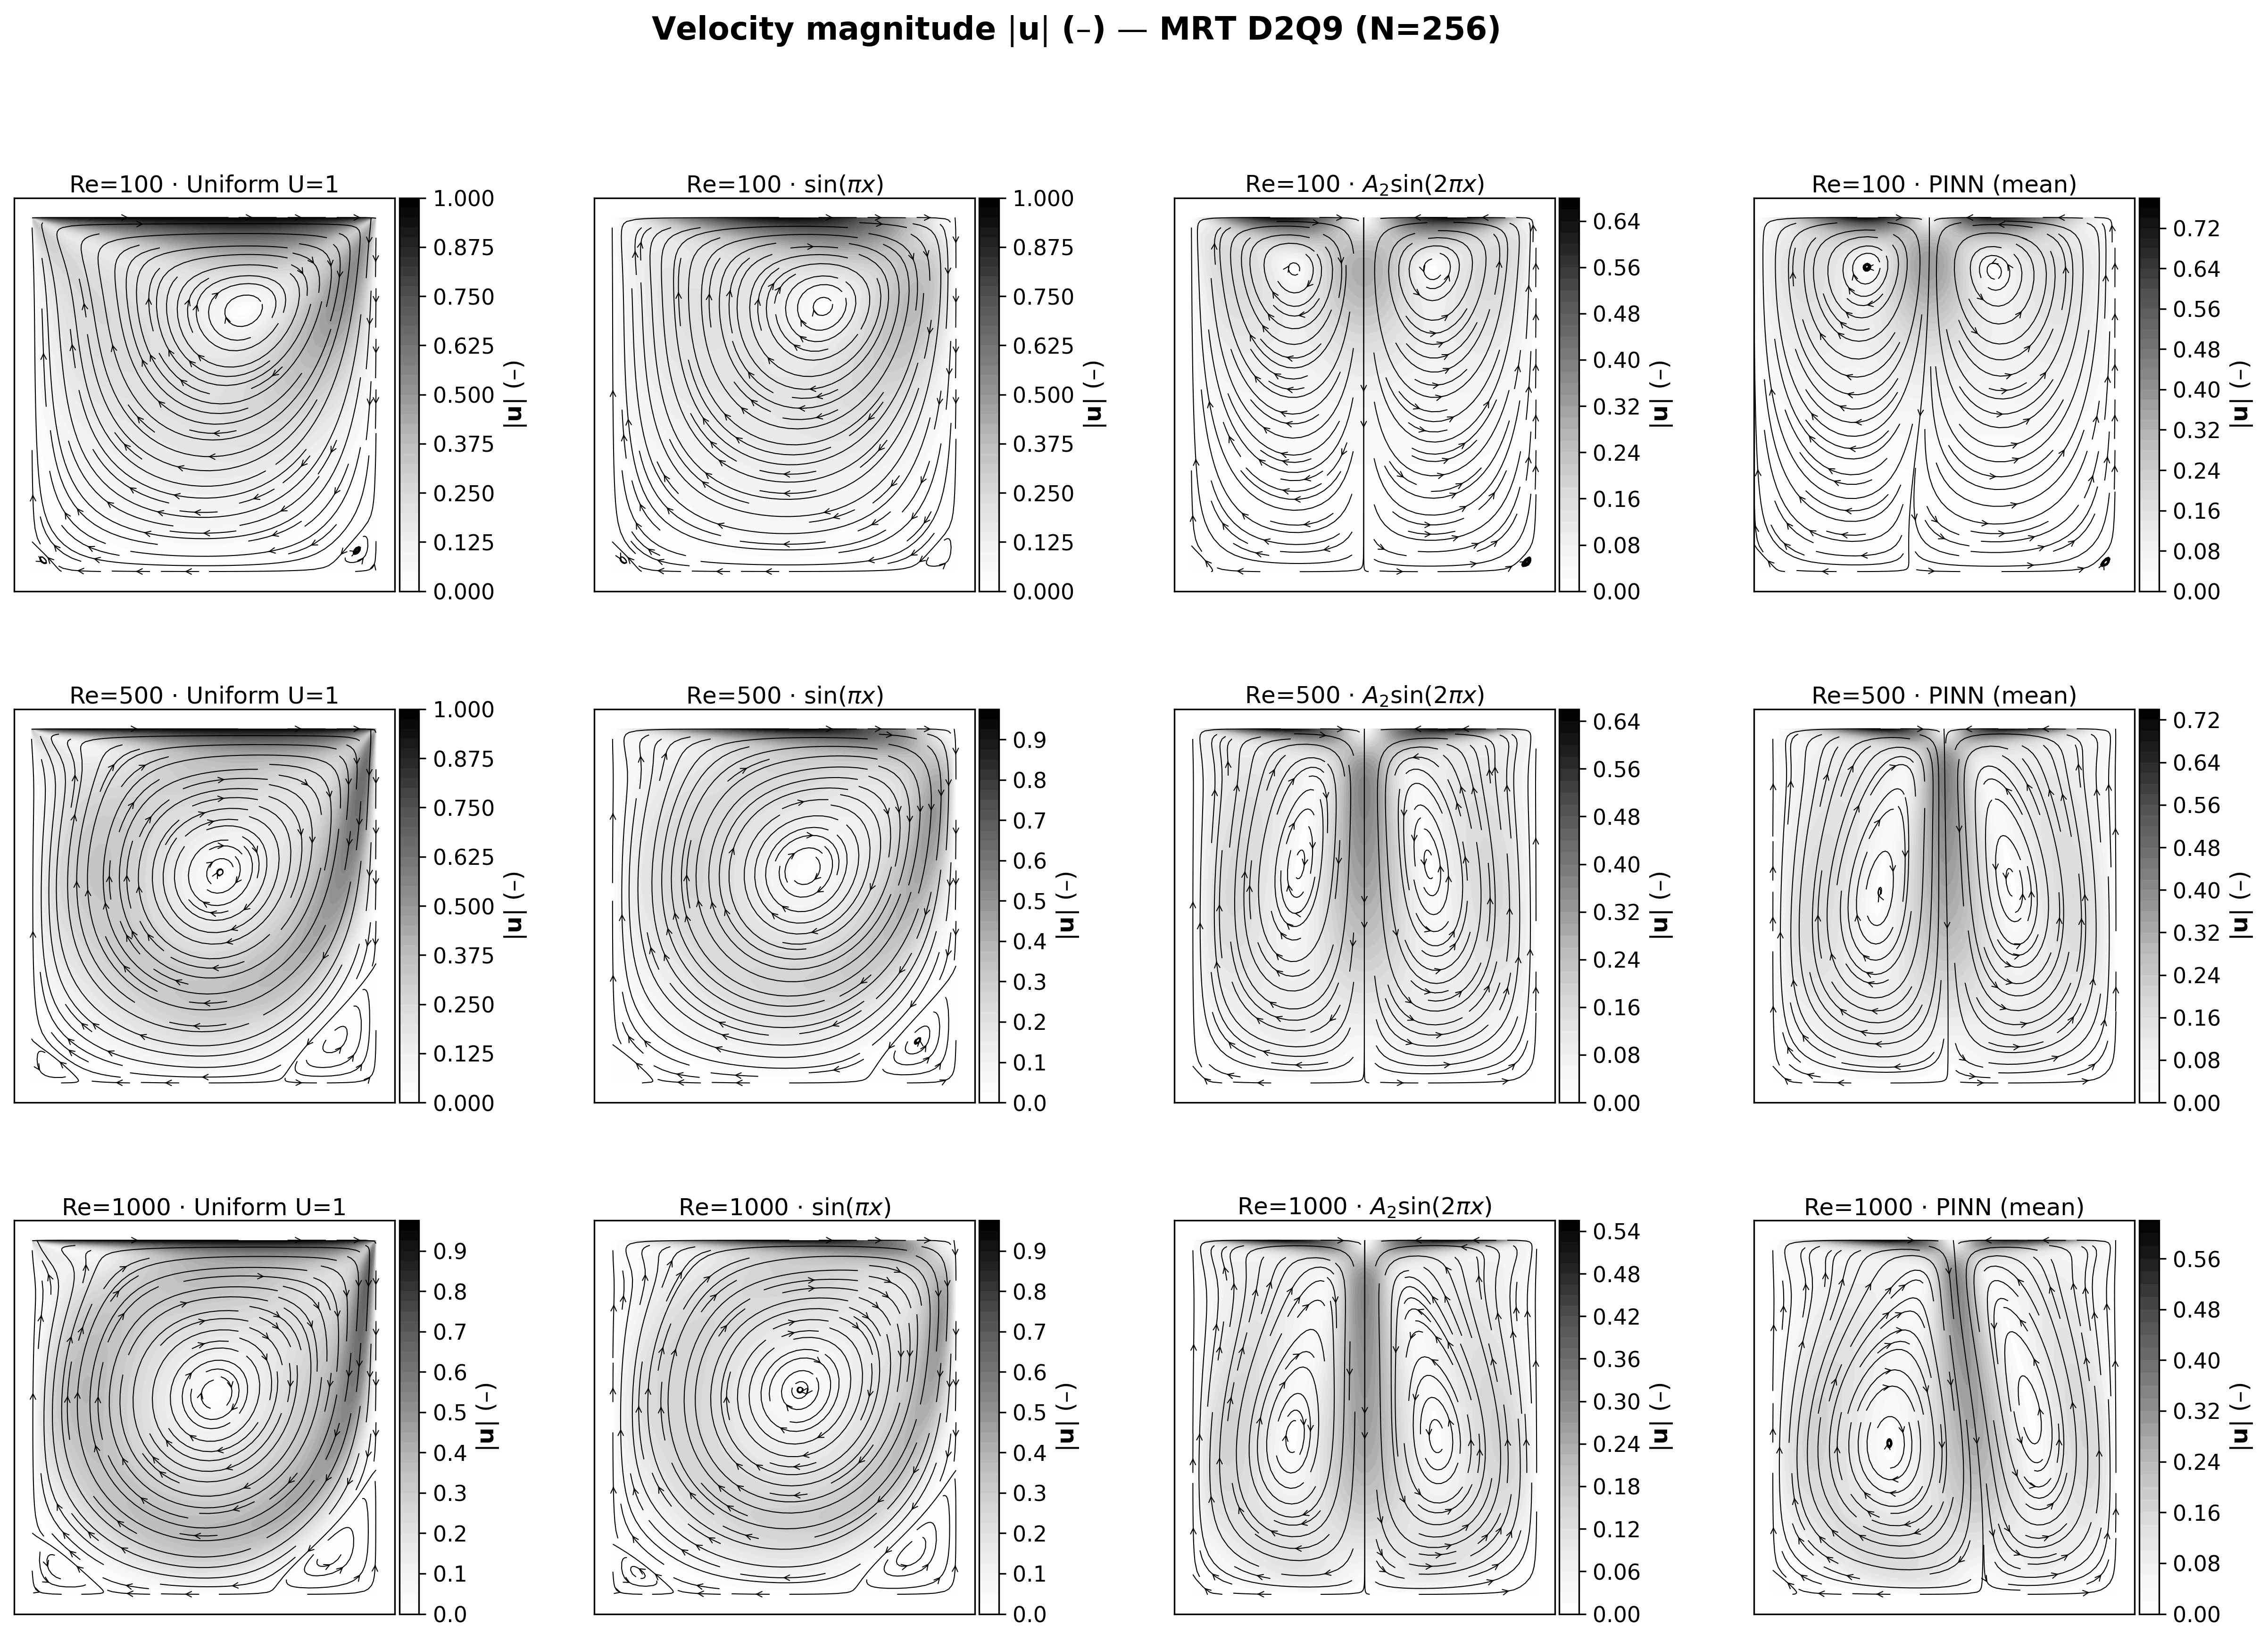
\includegraphics[width=0.8\textwidth]{figures/si_velocity_fields.png}
\caption{Velocity fields of the Fourier branch at $\re=100$, $500$, and $1000$ realized in the LBM solver. Color denotes the velocity magnitude; streamlines trace the central circulation set up by the dominant second spatial mode.}
\label{fig:s1}
\end{figure}

\begin{figure}[h]
\centering
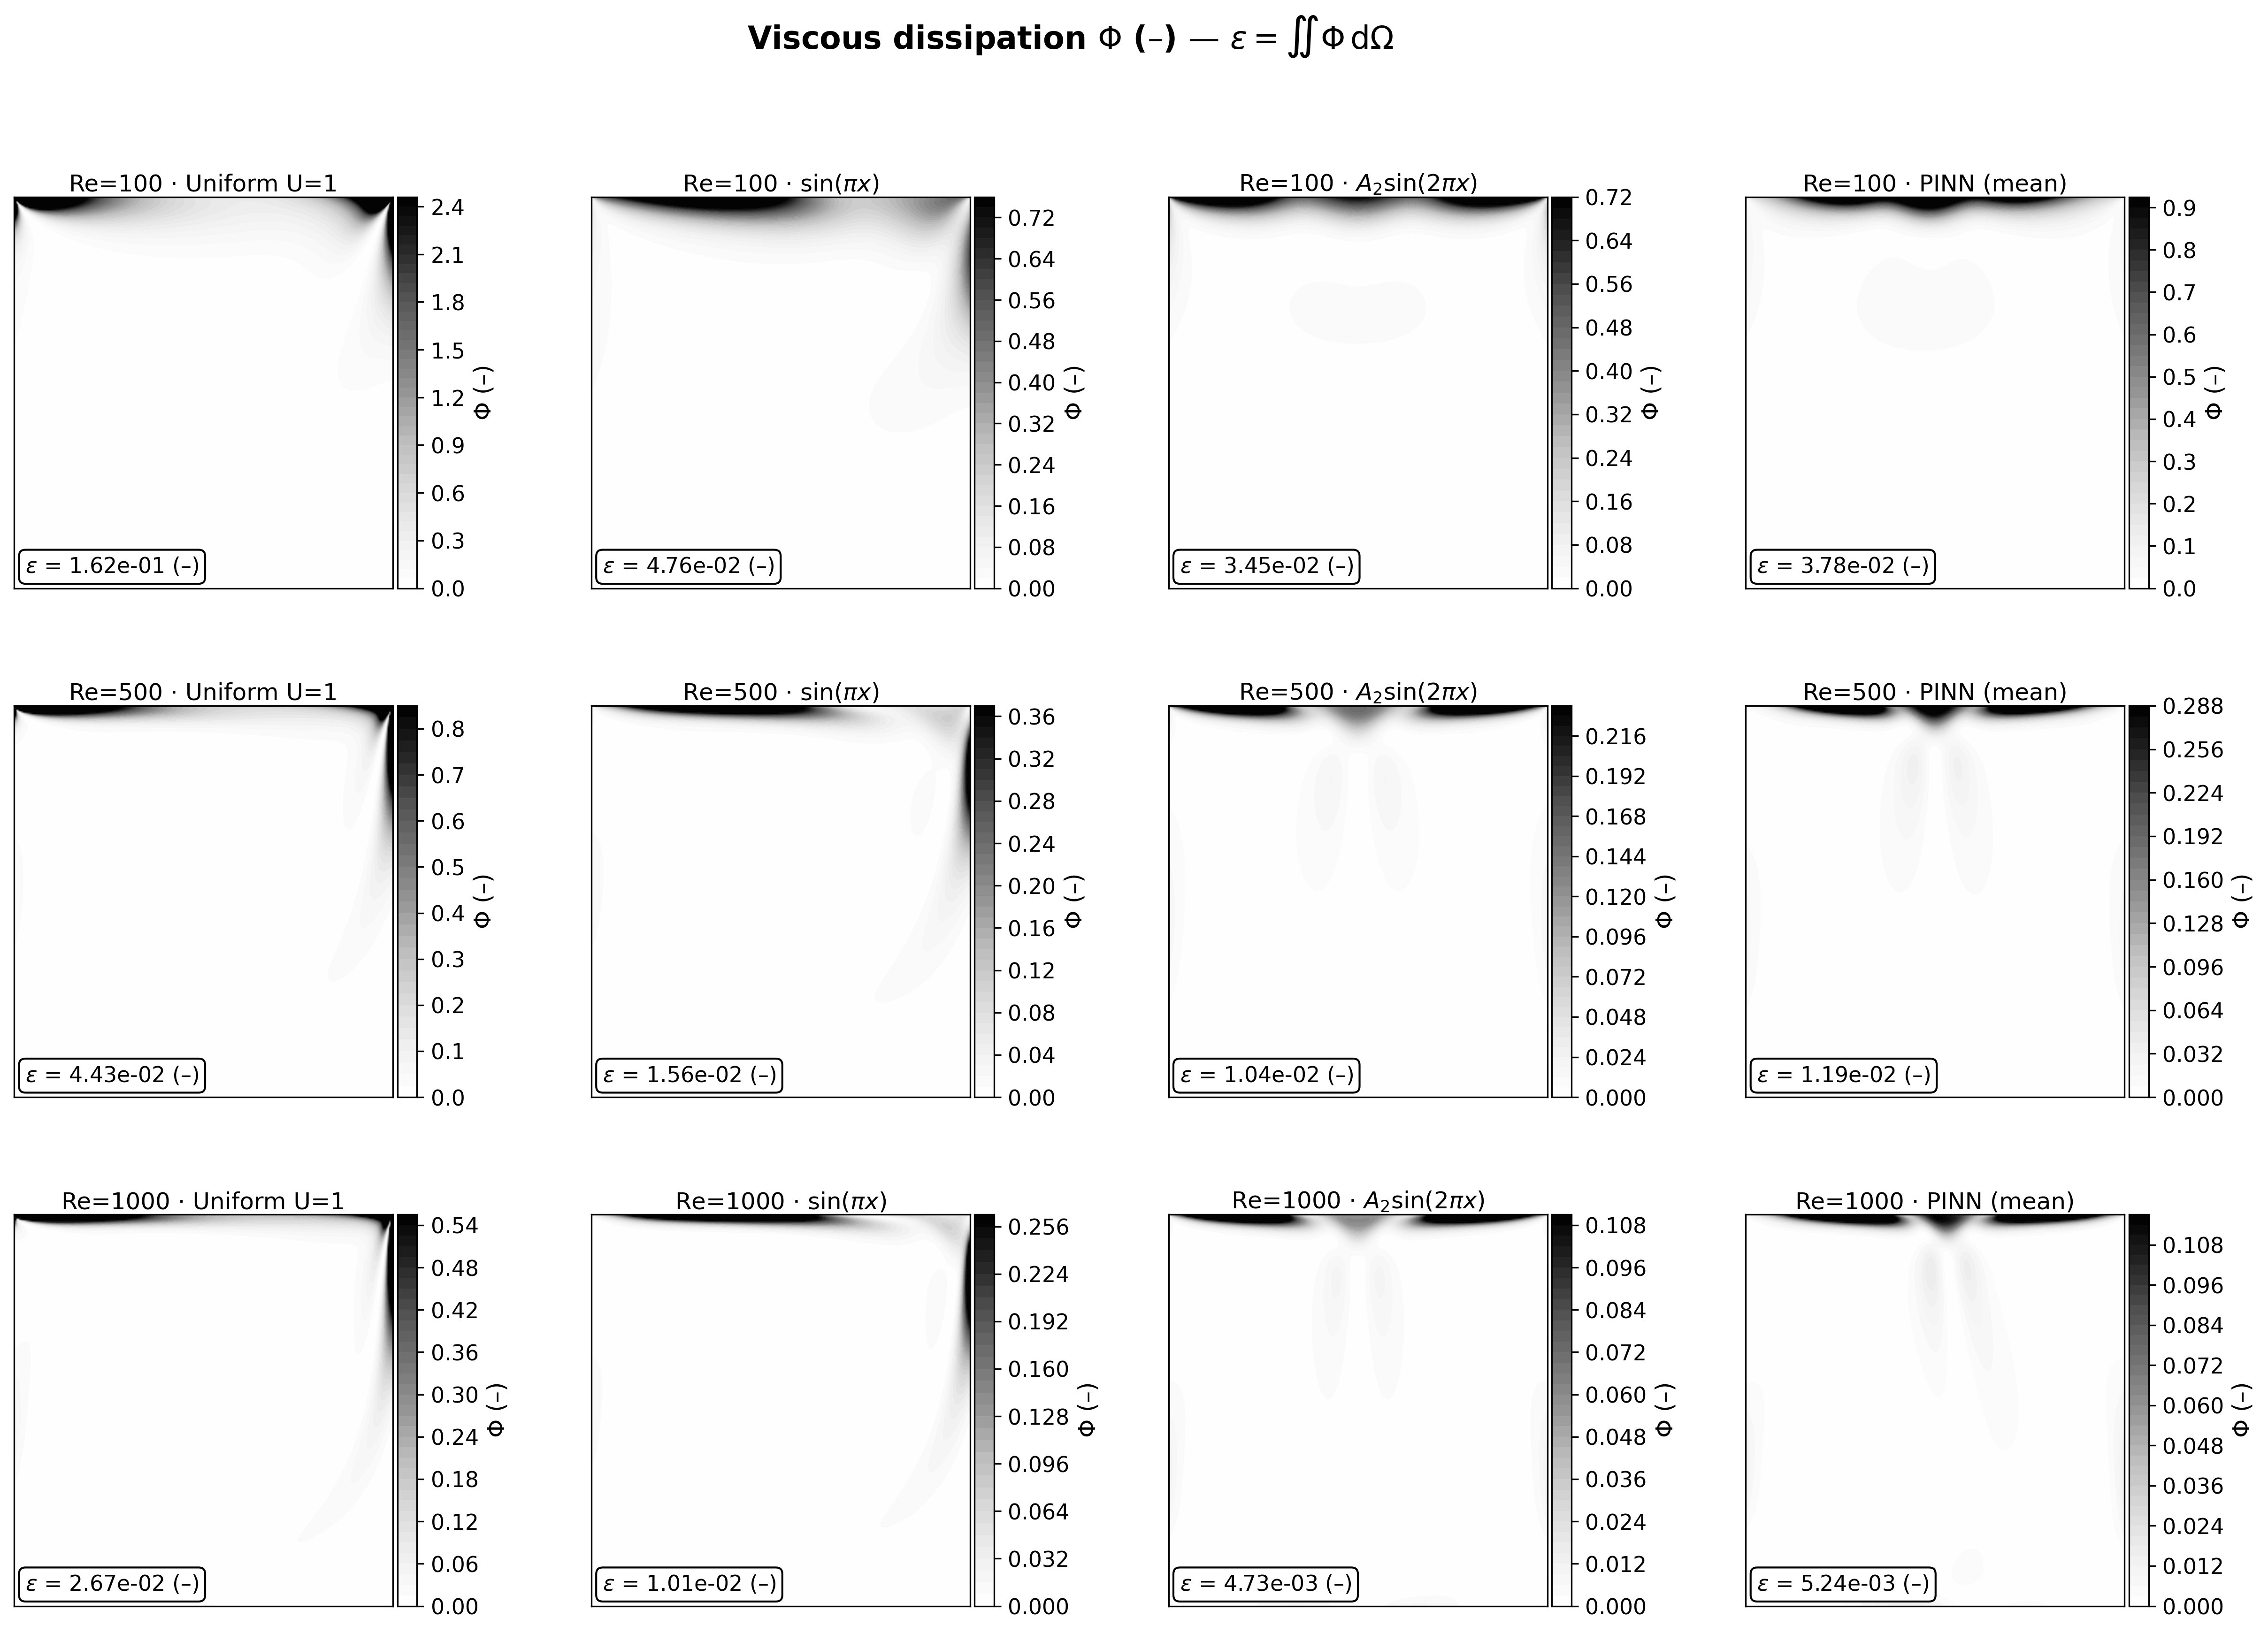
\includegraphics[width=0.8\textwidth]{figures/si_dissipation_fields.png}
\caption{Viscous dissipation fields of the Fourier branch at $\re=100$, $500$, and $1000$ realized in the LBM solver. The dissipation is concentrated in the shear layers set up by the forced motion.}
\label{fig:s2}
\end{figure}

\section{Modal content of the realized mean flows}

The main-text admissibility discussion refers to the modal content of the mean fields realized under the identified control. Figure~S3 reports the Fourier analysis of the vertical-centerline velocity $u(0.5,y)$ of the LBM-realized flows under the complete PINN control and its dominant-mode truncation $A_2\sin(2\pi x)$, at the three Reynolds numbers.

\begin{figure}[h]
\centering
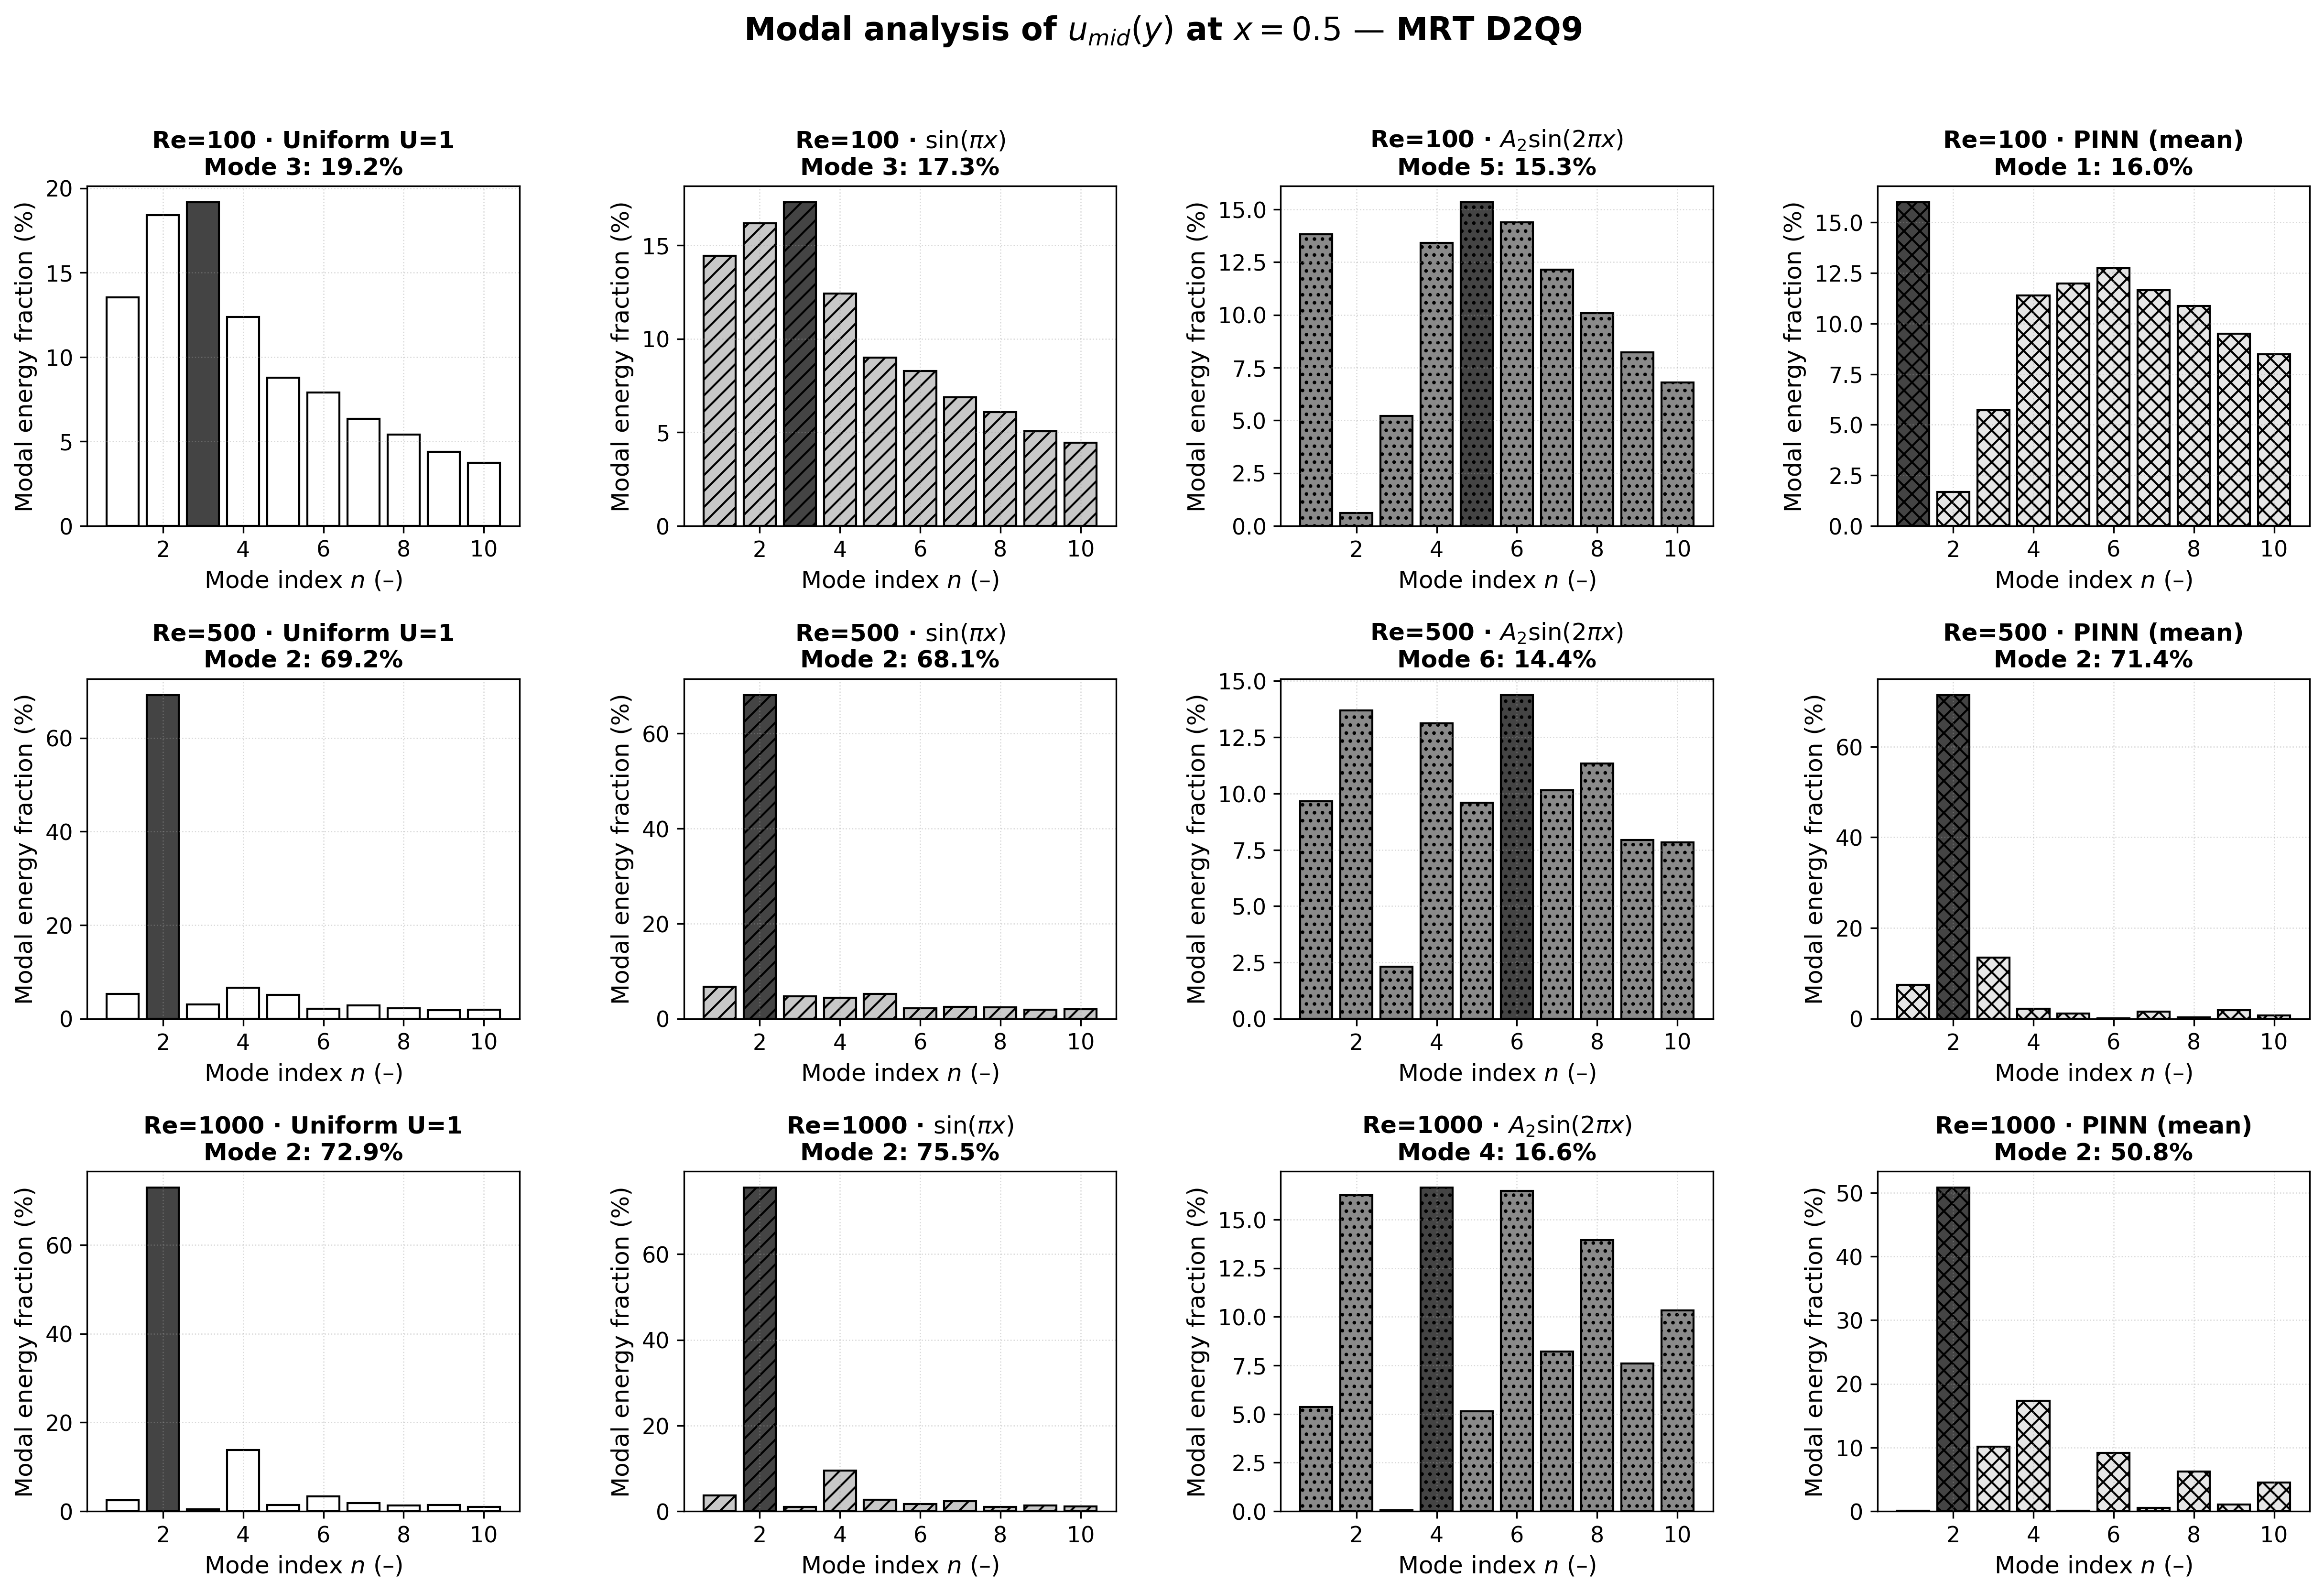
\includegraphics[width=0.8\textwidth]{figures/si_modal_analysis.png}
\caption{Modal analysis of the vertical-centerline velocity $u(0.5,y)$ of the LBM-realized flows under the PINN (mean) and $A_2\sin(2\pi x)$ lid profiles at $\re=100$, $500$, and $1000$. The mean flow of the Fourier branch is dominated by the second spatial contribution, consistent with the structure of the identified control.}
\label{fig:s3}
\end{figure}

\section{Centerline velocity profiles}

Figure~S4 shows the centerline velocity profiles of the realized flows under the four tested lid profiles at the three Reynolds numbers.

\begin{figure}[h]
\centering
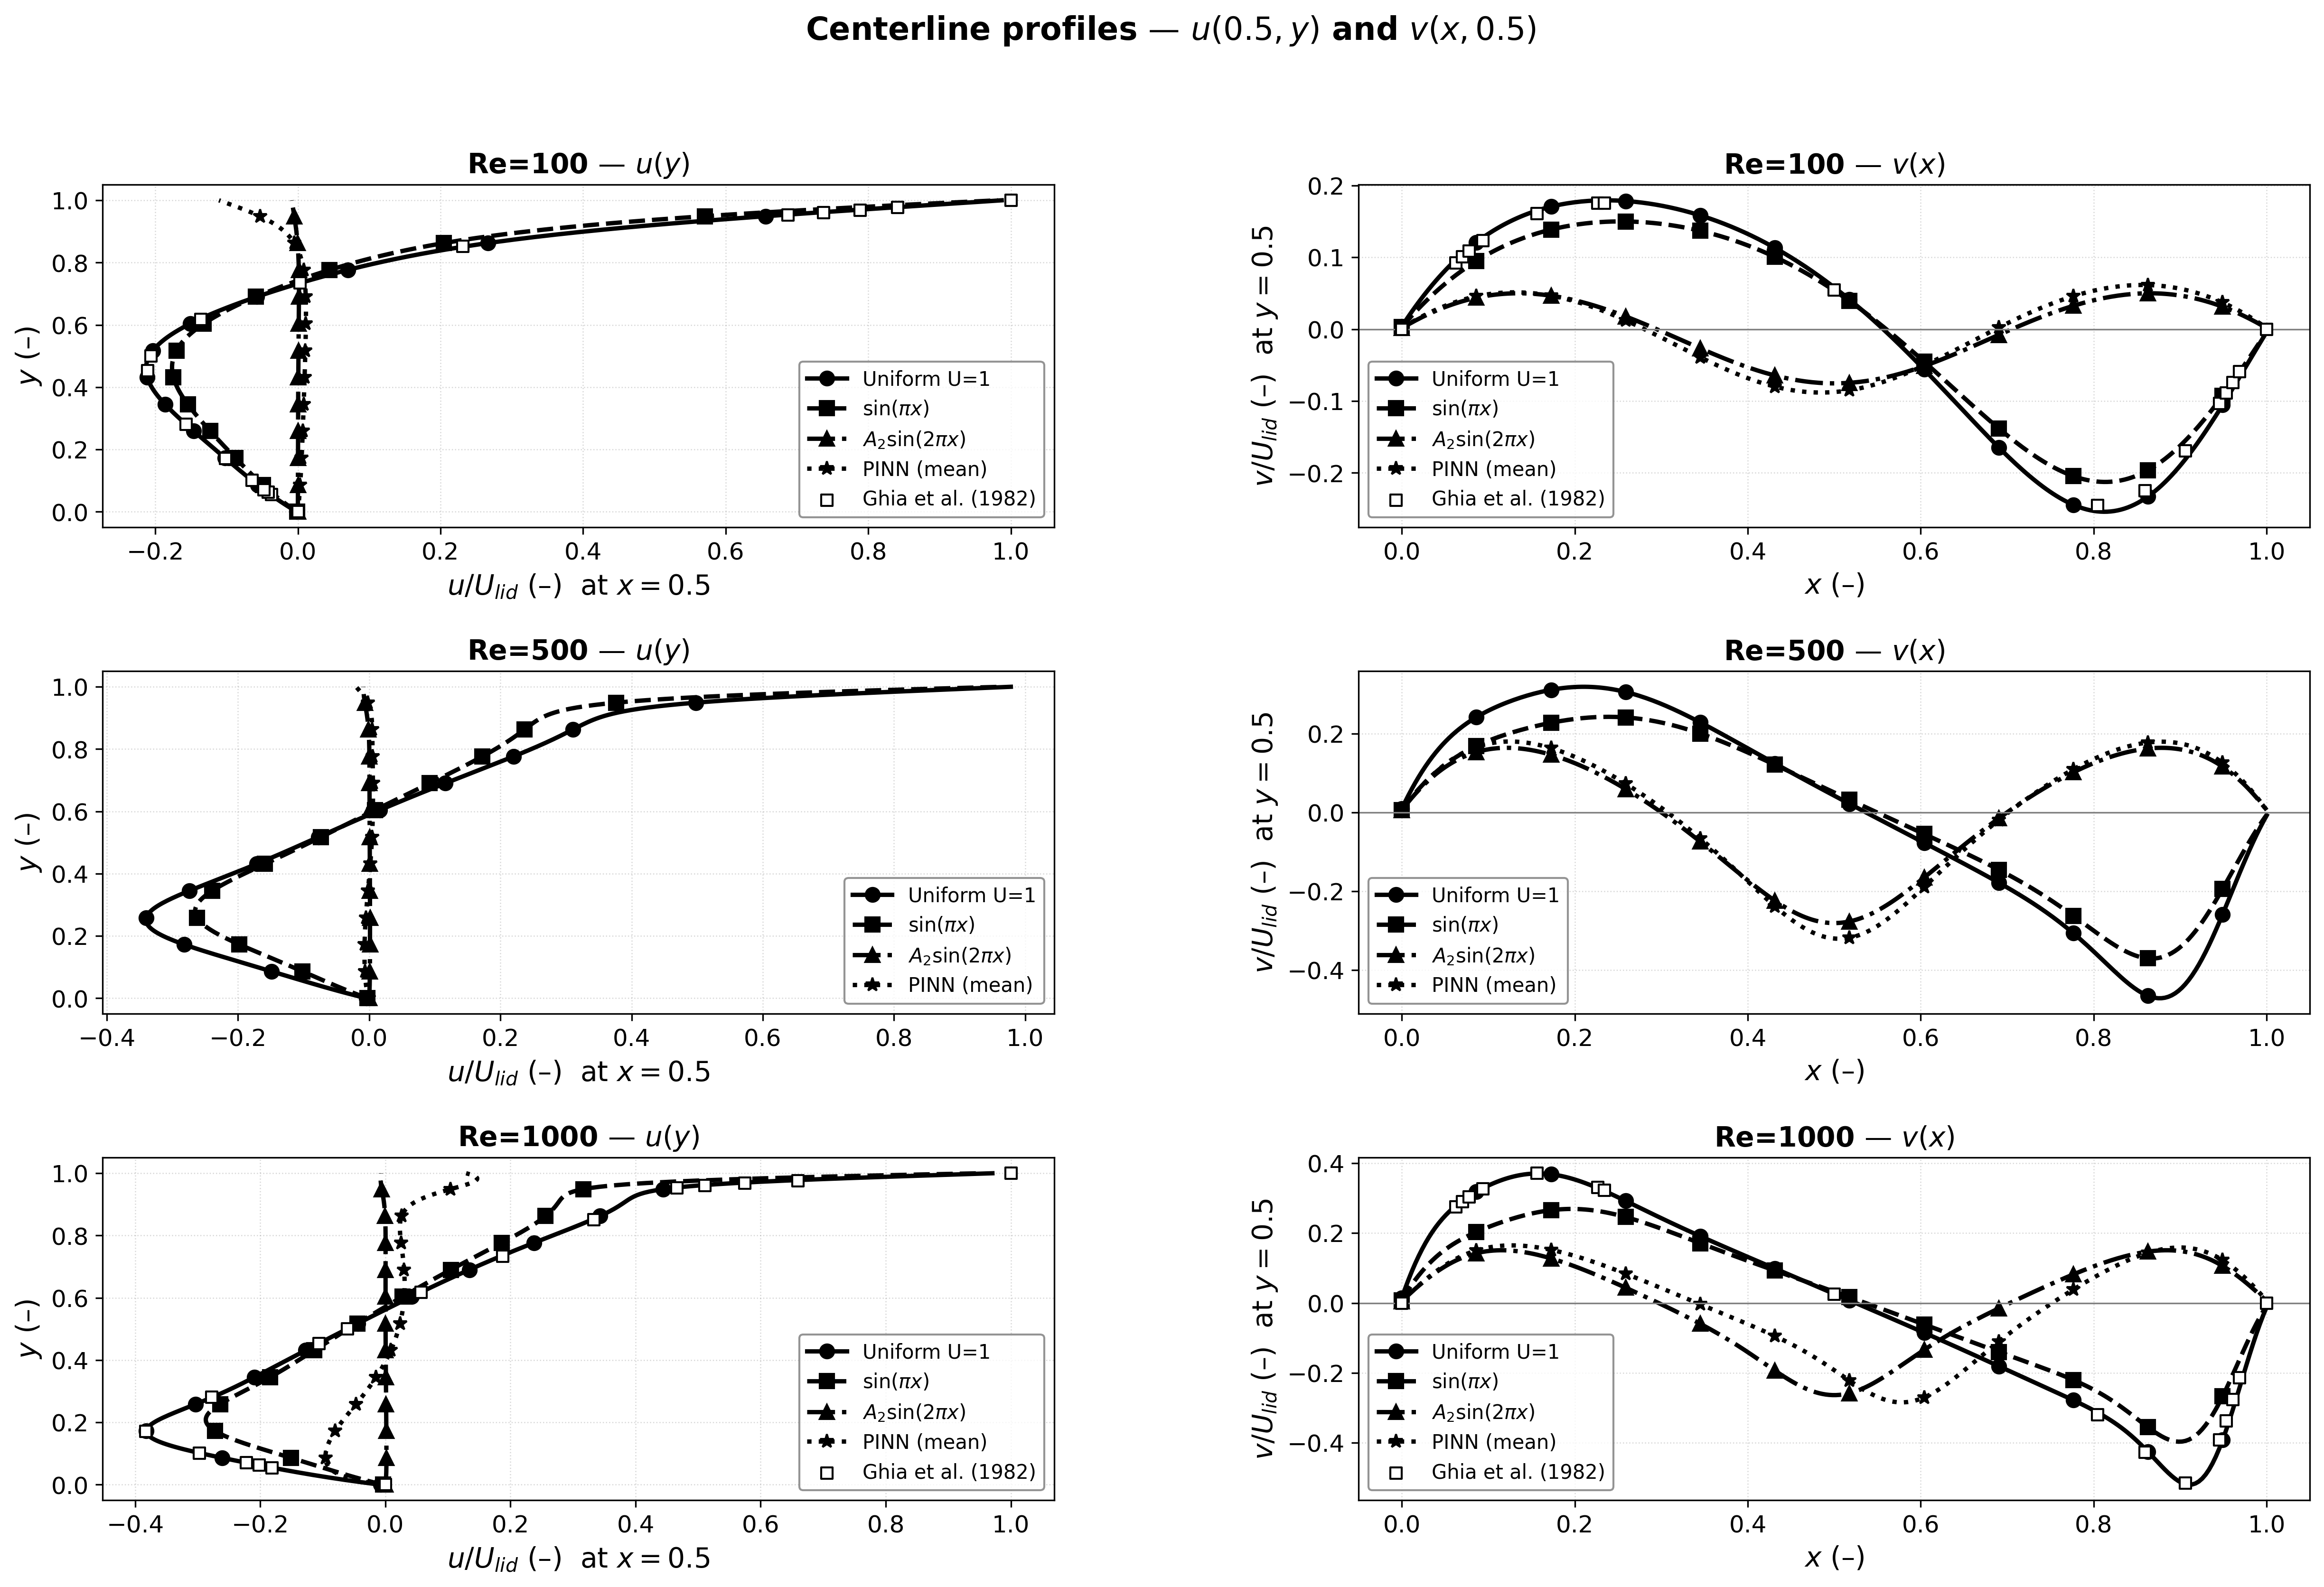
\includegraphics[width=0.8\textwidth]{figures/si_centerline_profiles.png}
\caption{Centerline velocity profiles $u(0.5,y)$ (left) and $v(x,0.5)$ (right) of the LBM-realized flows at $\re=100$, $500$, and $1000$, under the uniform, $\sin(\pi x)$, $A_2\sin(2\pi x)$, and PINN (mean) lid profiles.}
\label{fig:s4}
\end{figure}

\section{Modal spectra at $\re=100$, $500$, and $1000$}

Figures~S5--S7 show the spatial and temporal spectra of the recovered Fourier control at the three Reynolds numbers. In every case the second spatial mode is the largest individual contribution to the spatial spectrum; the temporal content is nearly flat at $\re=100$ and $500$ and becomes more pronounced at $\re=1000$, consistent with the main-text discussion of the mode-2 energy fraction.

\begin{figure}[h]
\centering
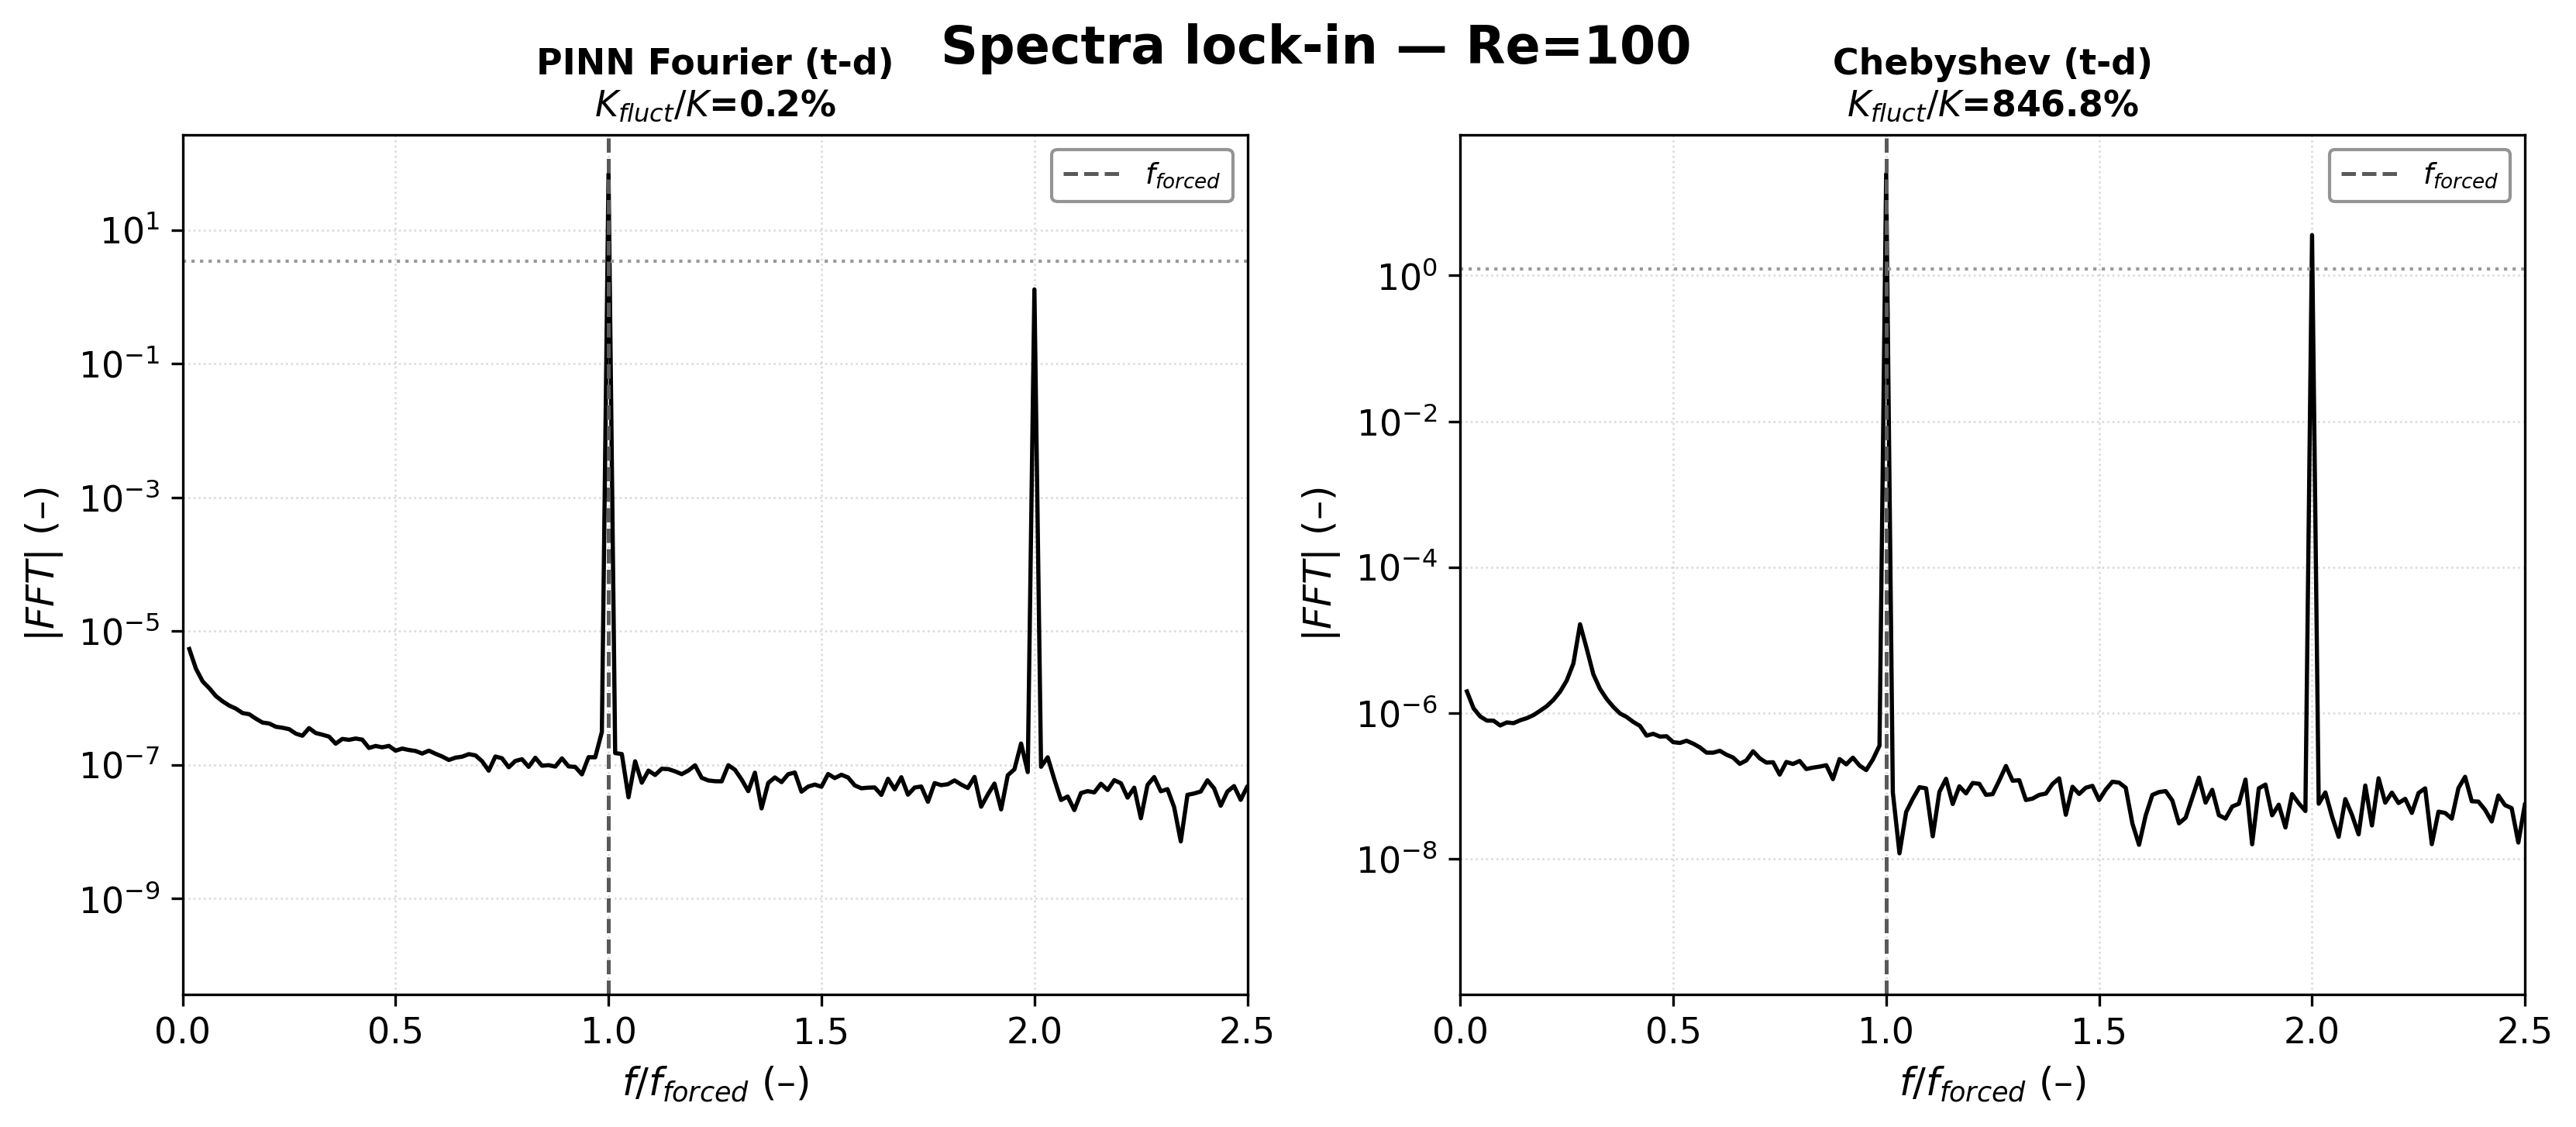
\includegraphics[width=0.8\textwidth]{figures/si_spectra_Re100.png}
\caption{Modal spectra of the recovered control at $\re=100$. The spatial spectrum is dominated by the second spatial mode; the temporal spectrum is essentially flat and small.}
\label{fig:s5}
\end{figure}

\begin{figure}[h]
\centering
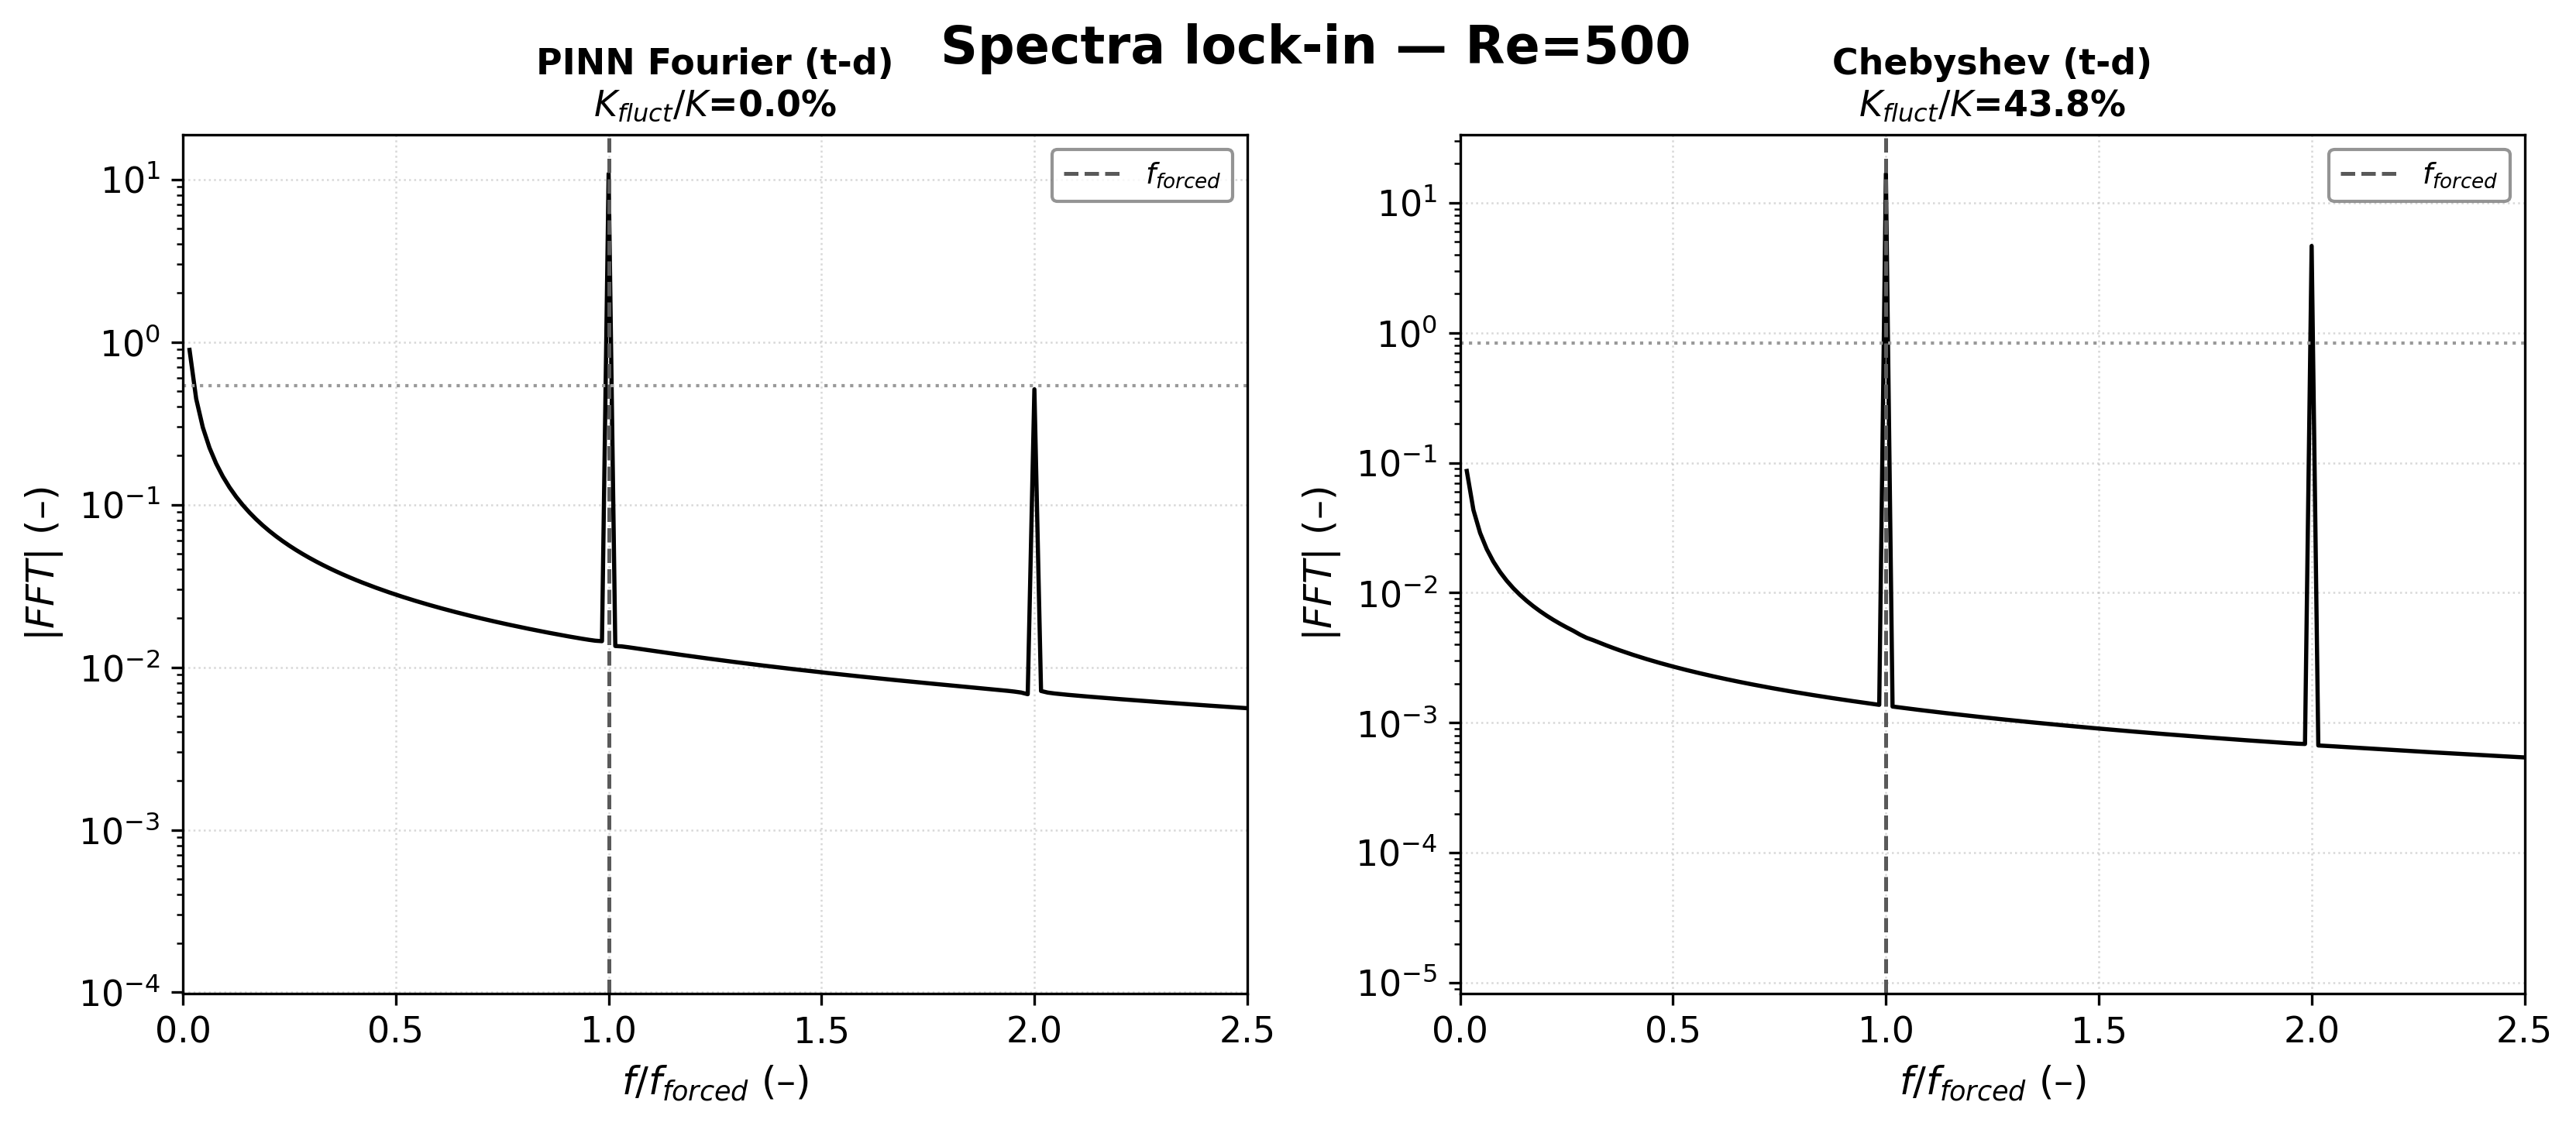
\includegraphics[width=0.8\textwidth]{figures/si_spectra_Re500.png}
\caption{Modal spectra of the recovered control at $\re=500$. The spatial spectrum still peaks at the second spatial mode with a small temporal content.}
\label{fig:s6}
\end{figure}

\begin{figure}[h]
\centering
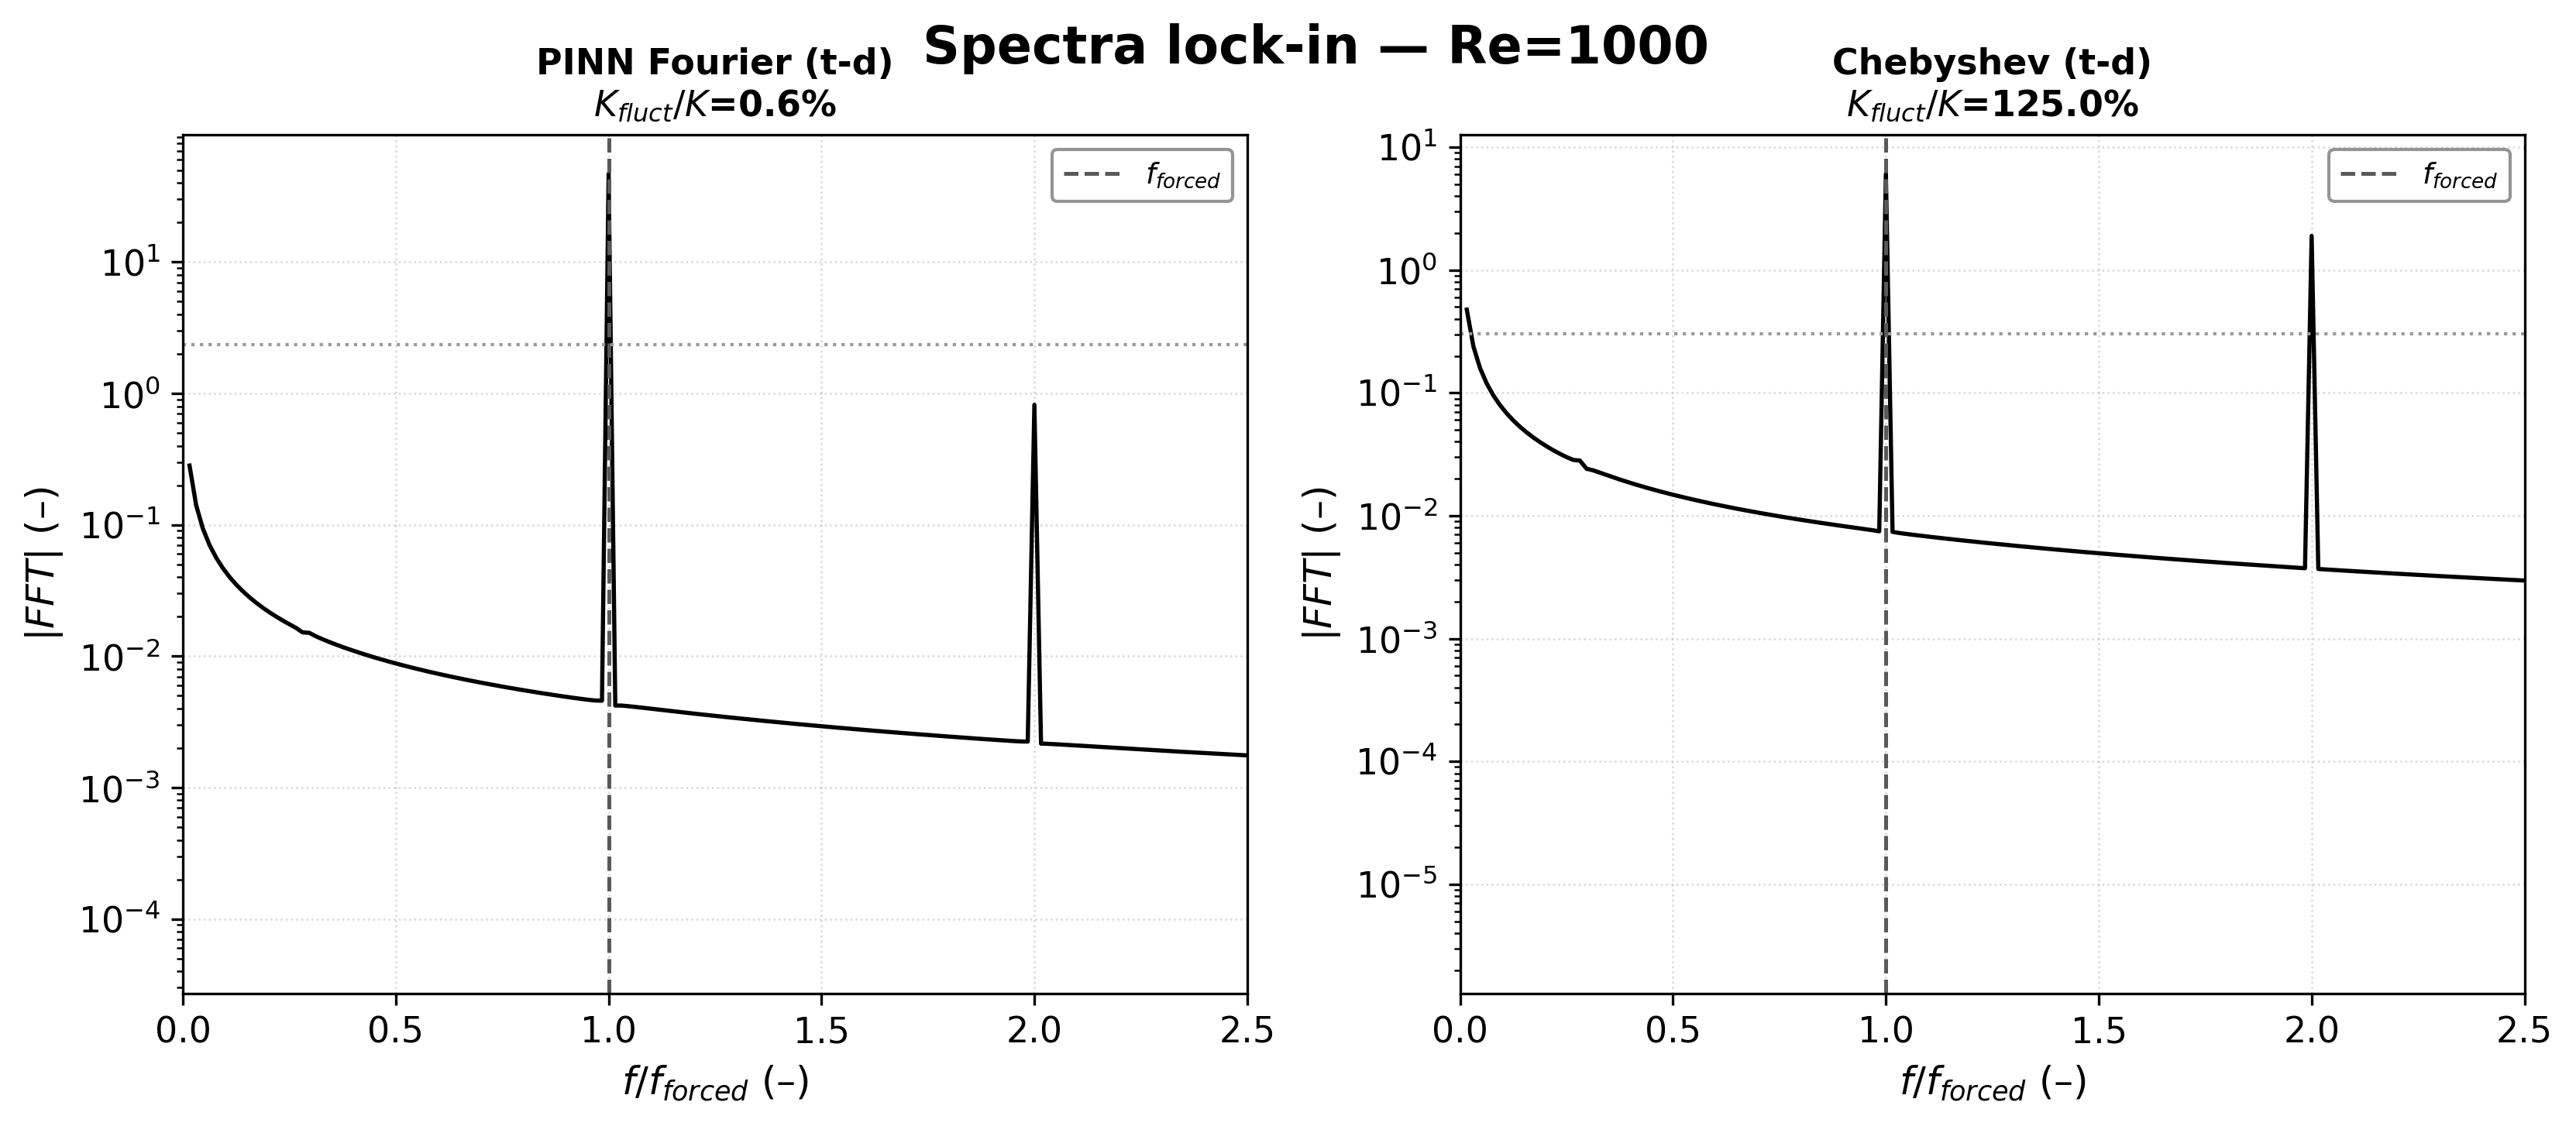
\includegraphics[width=0.8\textwidth]{figures/si_spectra_Re1000.png}
\caption{Modal spectra of the recovered control at $\re=1000$. The second spatial mode remains the largest individual spatial contribution, while the temporal content is more pronounced than at lower Reynolds number.}
\label{fig:s7}
\end{figure}

\section{Temporal response under the time-dependent Fourier control}

The admissibility test of the main text rests on the temporal behavior of the realized flows under the time-dependent ($t$-dependent) controls. Figures~S8--S10 show the LBM response to the periodic Fourier (PINN) control at the three Reynolds numbers: the fields at the phase of maximum forcing, a probe time series of the kinetic energy, and the spectra of the fluctuation content. The realizations are quasi-stationary: the fluctuation amplitude remains below $1\%$ of the mean-flow kinetic energy at every Reynolds number. Table~S2 reports the kinetic-energy diagnostics of these realizations and of the modified-Chebyshev ones. The very large ratio $R_K=847\%$ at $\re=100$ for the Chebyshev control originates from the small denominator $K_{\mathrm{mean}}\simeq9\times10^{-5}$, about two orders of magnitude below the Fourier values, rather than from an anomalously large fluctuation amplitude.

\begin{table}[h]
\centering
\caption{Kinetic-energy diagnostics of the LBM realizations under the time-dependent Fourier (PINN) and modified-Chebyshev controls at $\re=100$, $500$, and $1000$. $K_{\mathrm{mean}}$: kinetic energy of the time-averaged flow; $K_{\mathrm{fluct}}$: time-averaged fluctuation kinetic energy; $R_K=K_{\mathrm{fluct}}/K_{\mathrm{mean}}$.}
\label{tab:s2}
\begin{tabular}{lcccc}
\toprule
Control & $\re$ & $K_{\mathrm{mean}}$ & $K_{\mathrm{fluct}}$ & $R_K$ (\%) \\
\midrule
\multirow{3}{*}{PINN (Fourier, $t$-dependent)}
 & 100  & $8.34\times10^{-3}$ & $1.28\times10^{-5}$ & 0.15 \\
 & 500  & $1.17\times10^{-2}$ & $4.89\times10^{-6}$ & 0.04 \\
 & 1000 & $8.33\times10^{-3}$ & $5.41\times10^{-5}$ & 0.65 \\
\addlinespace
\multirow{3}{*}{Chebyshev ($t$-dependent)}
 & 100  & $9.02\times10^{-5}$ & $7.63\times10^{-4}$ & 847 \\
 & 500  & $5.48\times10^{-4}$ & $2.40\times10^{-4}$ & 44.0 \\
 & 1000 & $1.30\times10^{-4}$ & $1.62\times10^{-4}$ & 125 \\
\bottomrule
\end{tabular}
\end{table}

\begin{figure}[h]
\centering
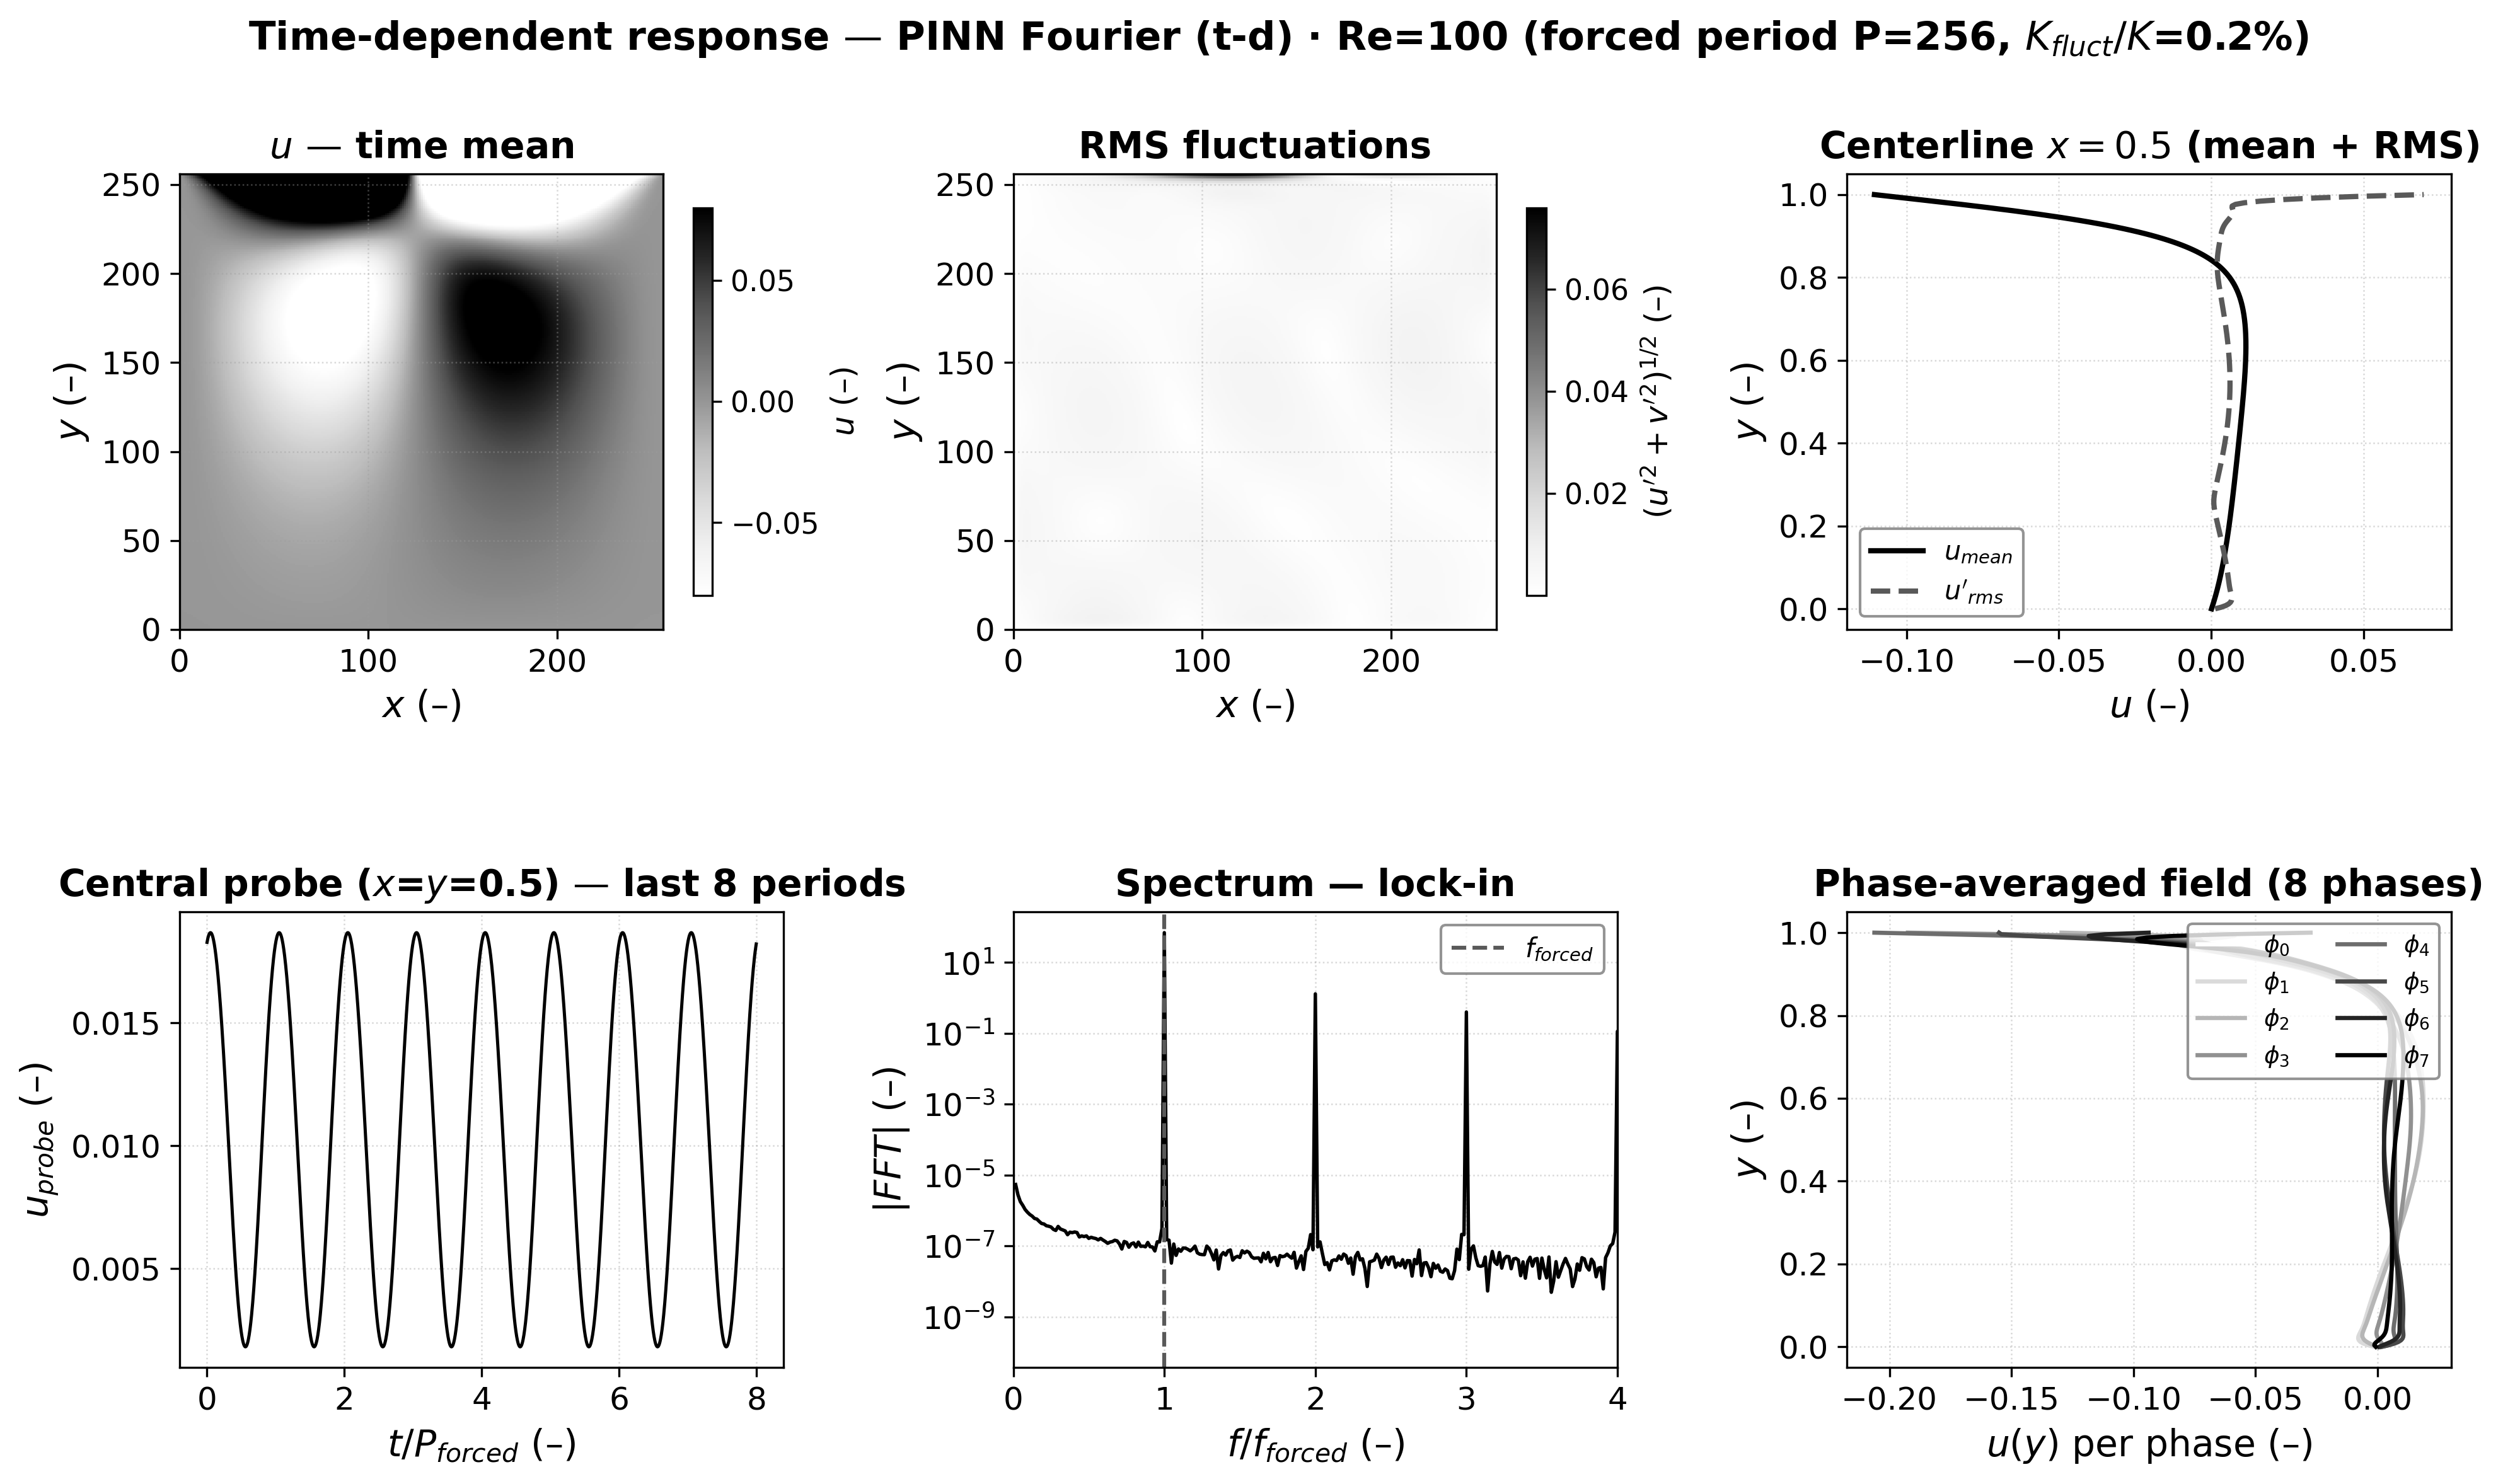
\includegraphics[width=0.8\textwidth]{figures/si_pinn_t_Re100.png}
\caption{Temporal response of the LBM realization to the time-dependent Fourier (PINN) control at $\re=100$.}
\label{fig:s8}
\end{figure}

\begin{figure}[h]
\centering
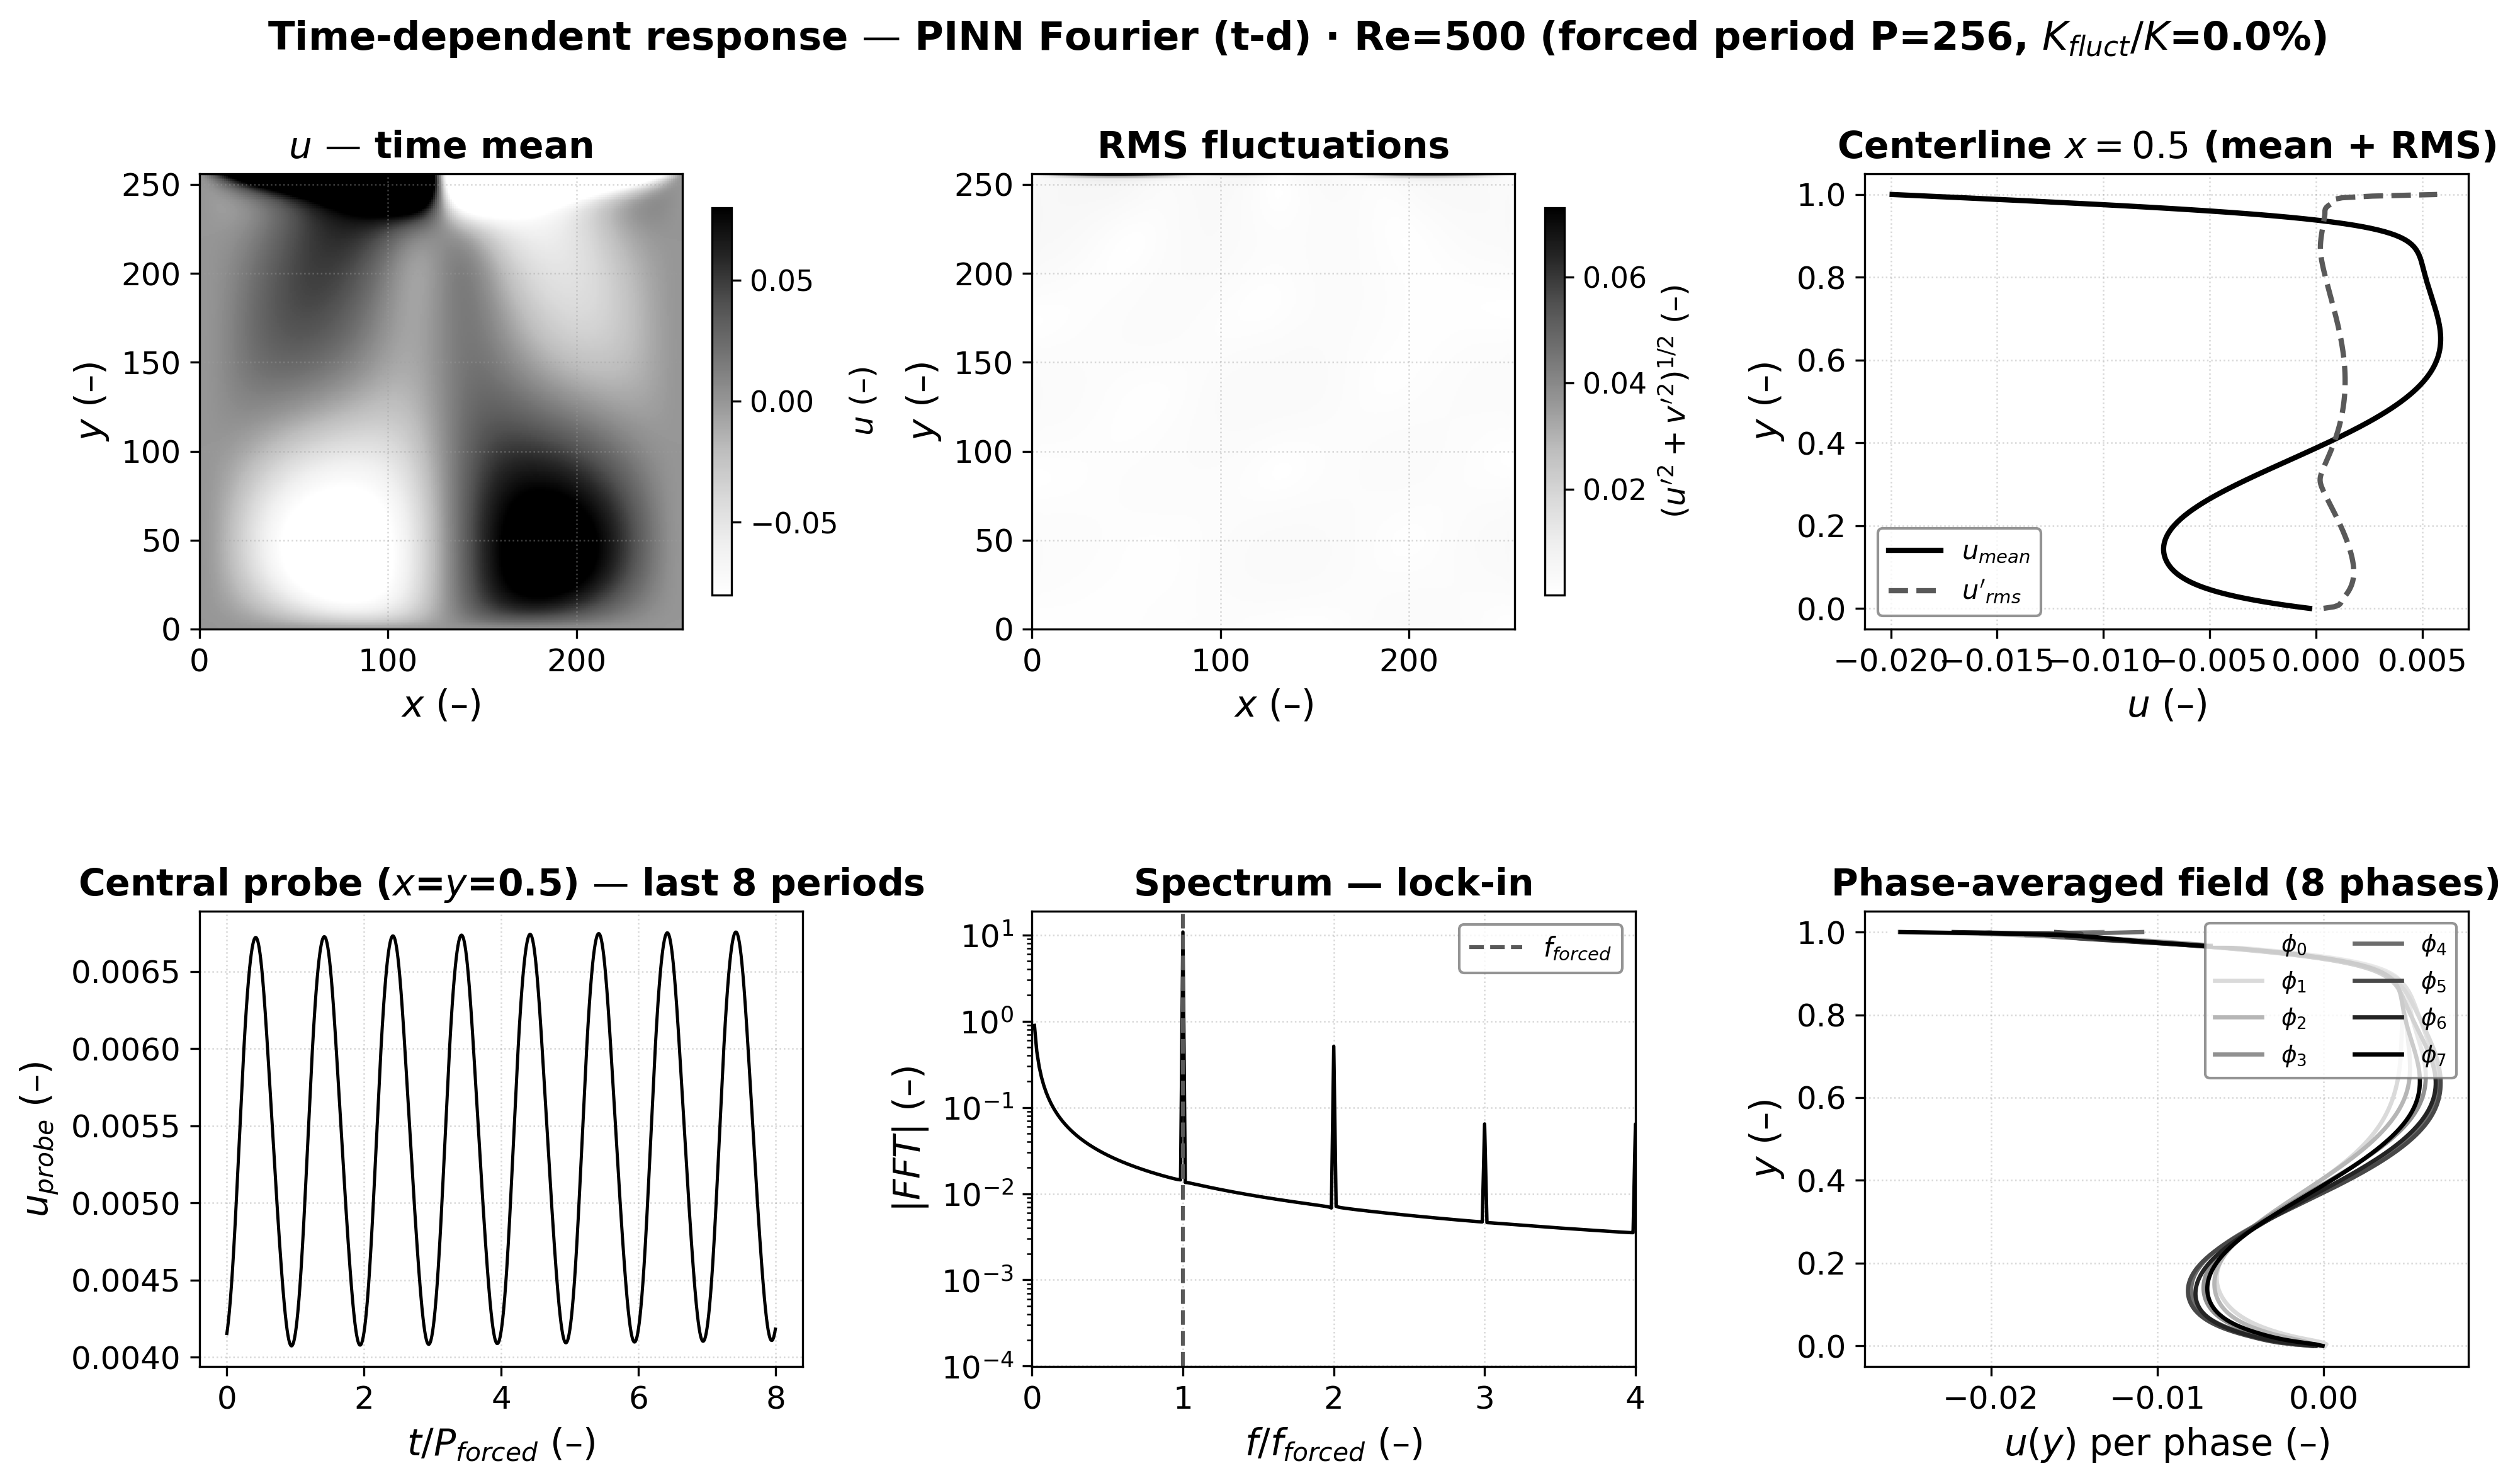
\includegraphics[width=0.8\textwidth]{figures/si_pinn_t_Re500.png}
\caption{Temporal response of the LBM realization to the time-dependent Fourier (PINN) control at $\re=500$.}
\label{fig:s9}
\end{figure}

\begin{figure}[h]
\centering
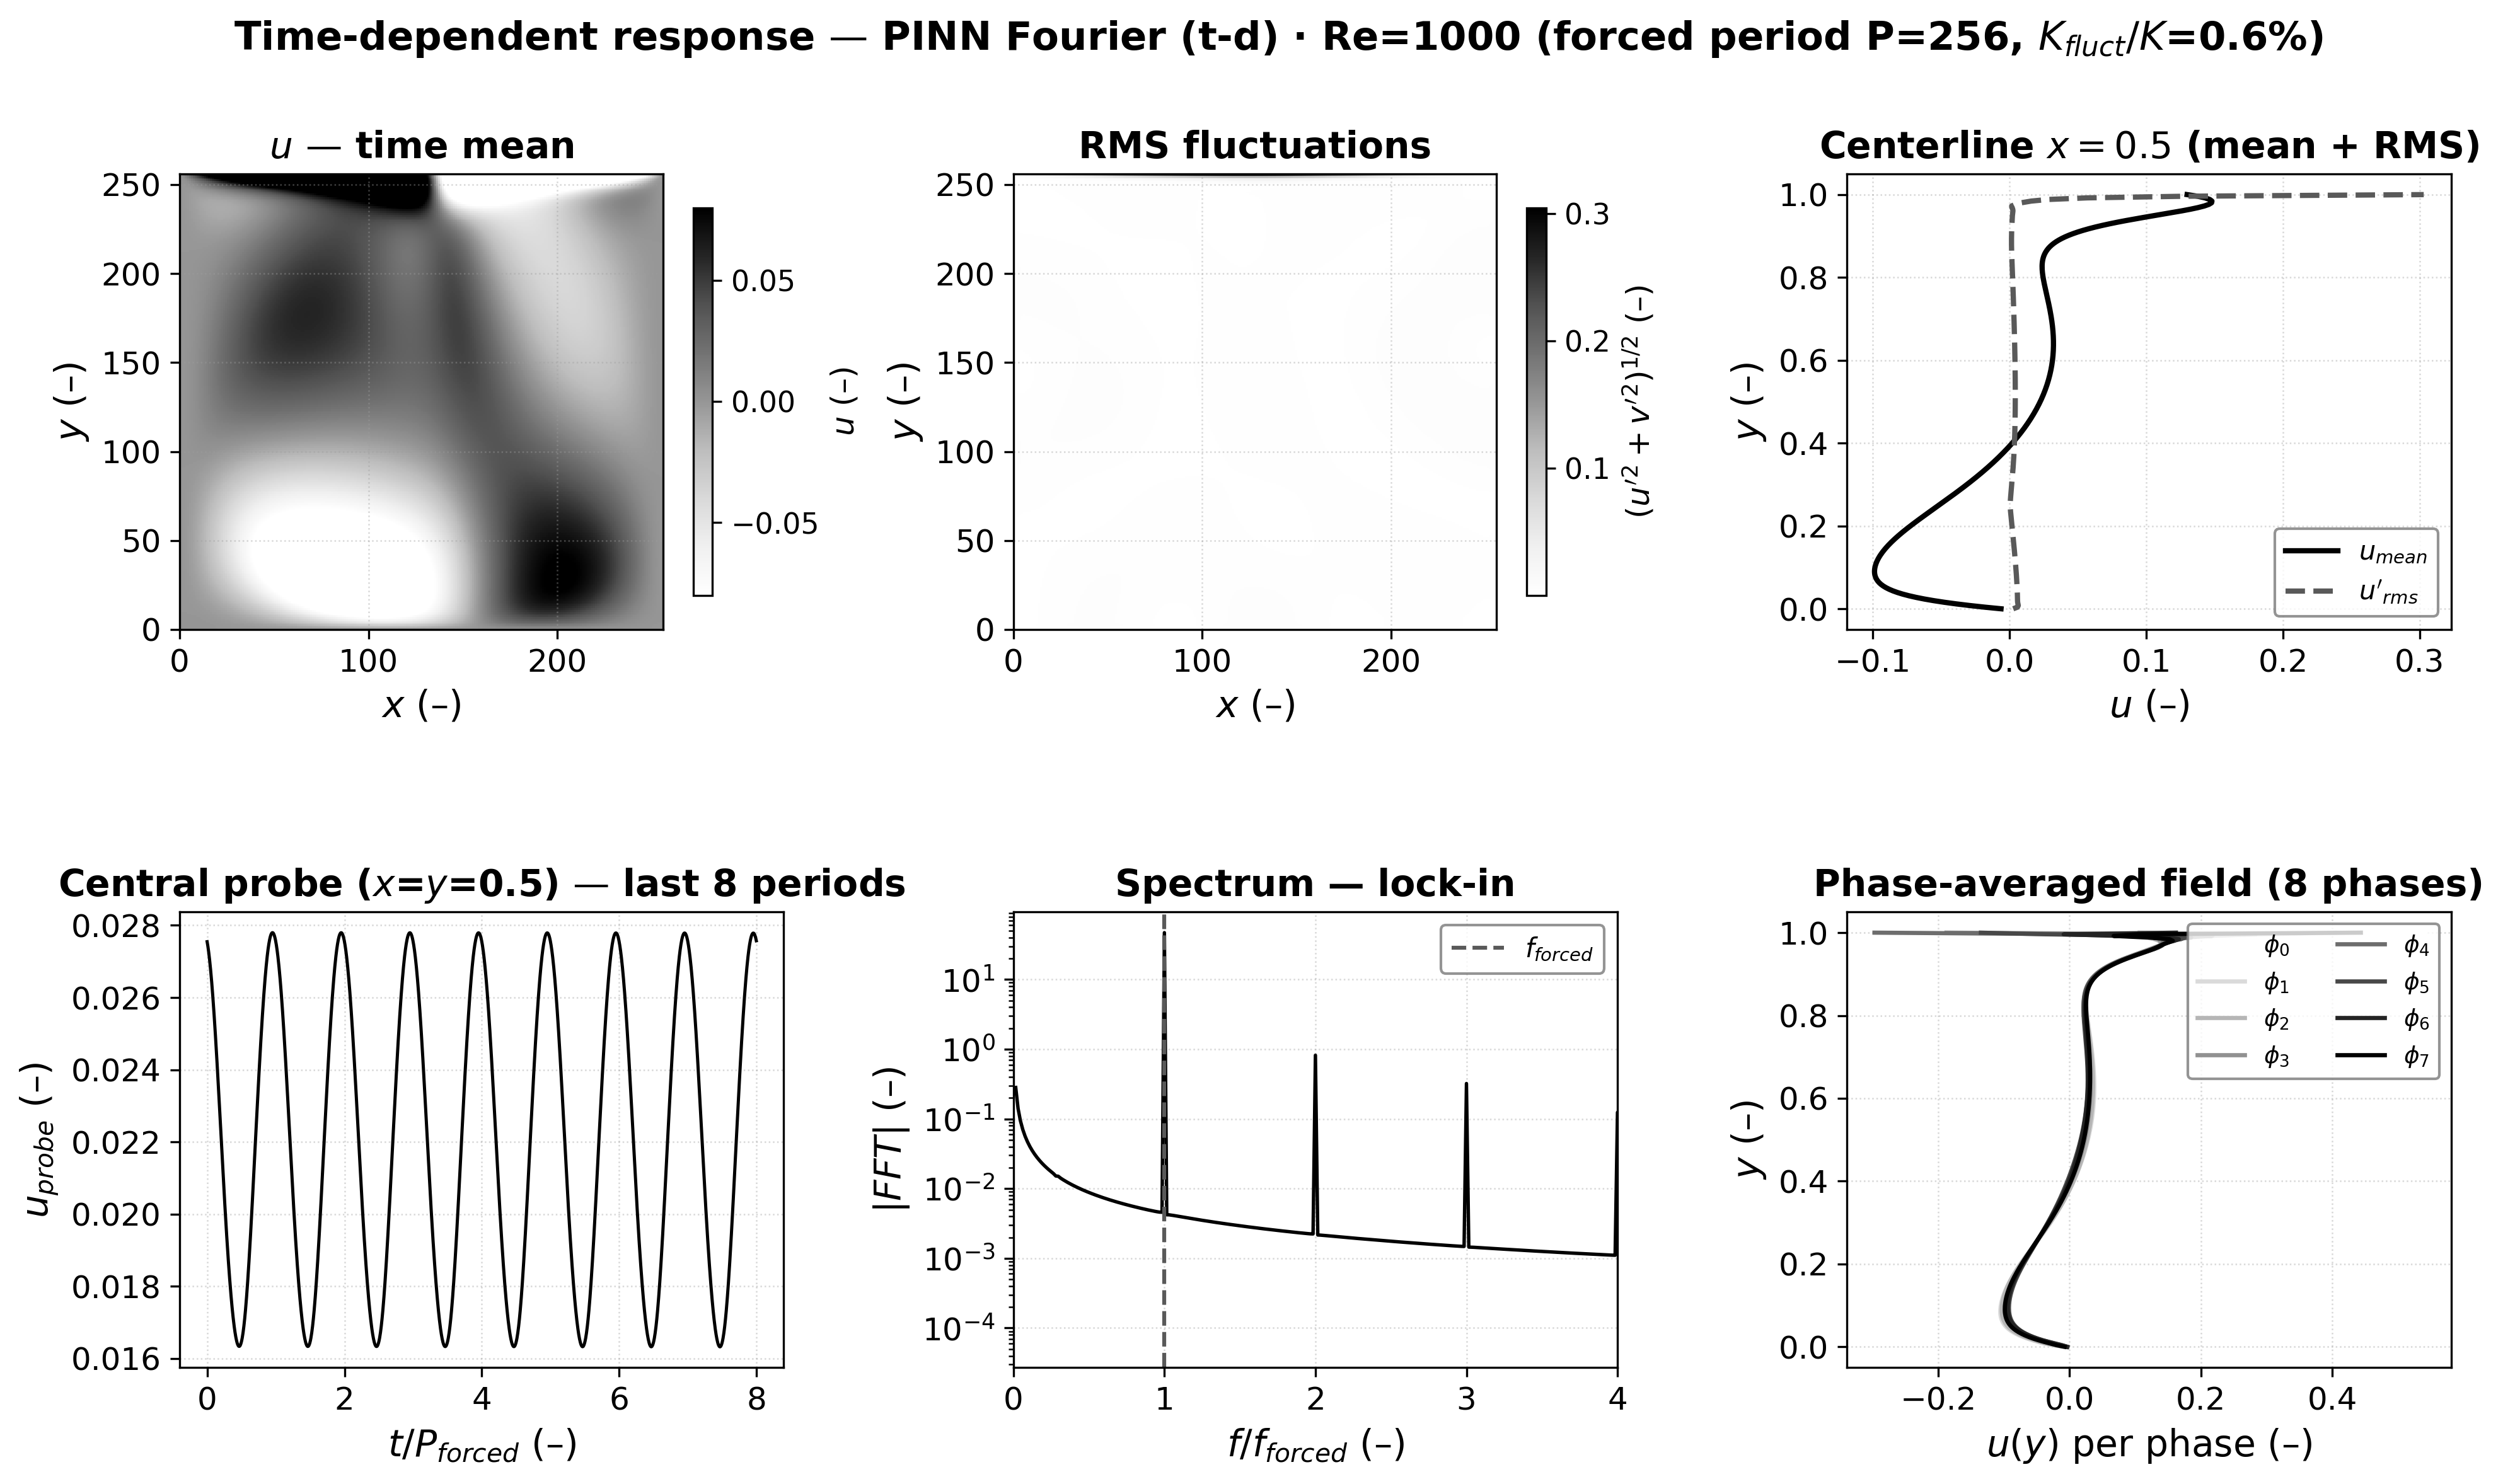
\includegraphics[width=0.8\textwidth]{figures/si_pinn_t_Re1000.png}
\caption{Temporal response of the LBM realization to the time-dependent Fourier (PINN) control at $\re=1000$.}
\label{fig:s10}
\end{figure}

\section{Temporal response to the time-dependent modified-Chebyshev control}

Figures~S11--S13 show the corresponding realization under the time-dependent modified-Chebyshev control. In contrast to the Fourier case, the fluctuations dominate the kinetic energy at every Reynolds number, and the realized mean-flow kinetic energy is small relative to the fluctuation contribution (Table~S2). These runs provide the quantitative basis of the failure of this branch under the adopted admissibility test.

\begin{figure}[h]
\centering
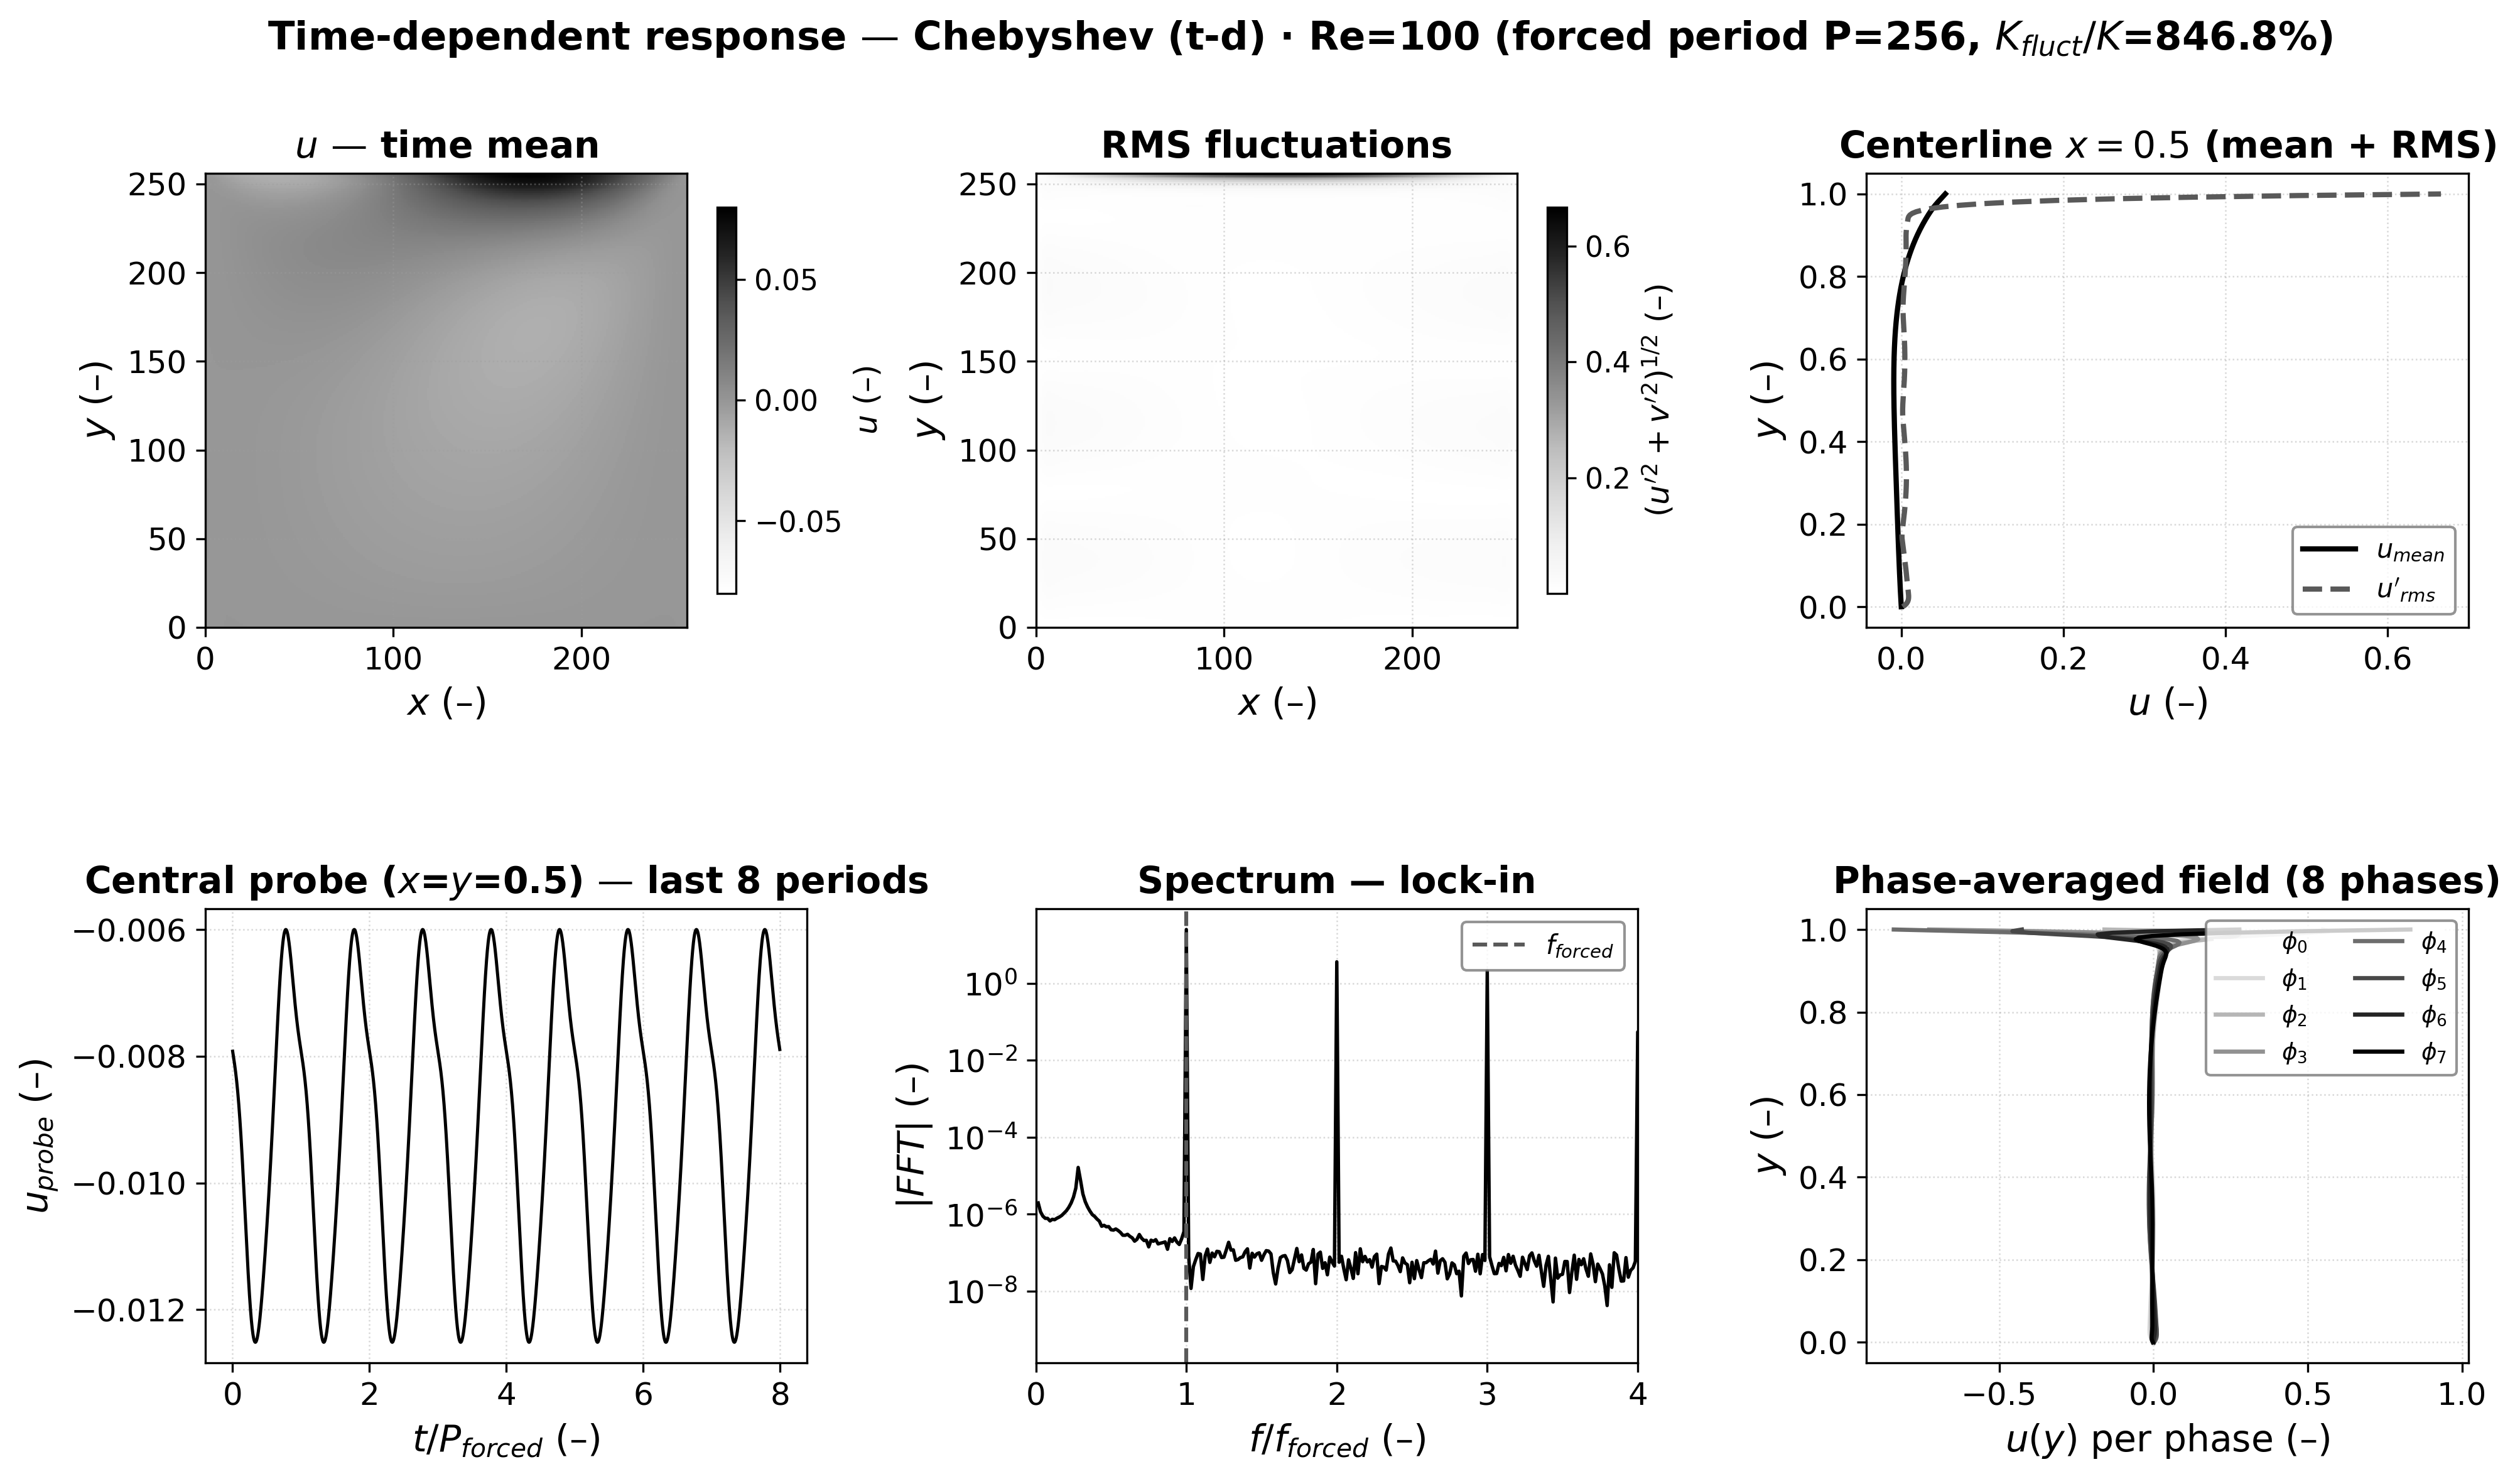
\includegraphics[width=0.8\textwidth]{figures/si_cheb_t_Re100.png}
\caption{Temporal response of the LBM realization to the time-dependent modified-Chebyshev control at $\re=100$.}
\label{fig:s11}
\end{figure}

\begin{figure}[h]
\centering
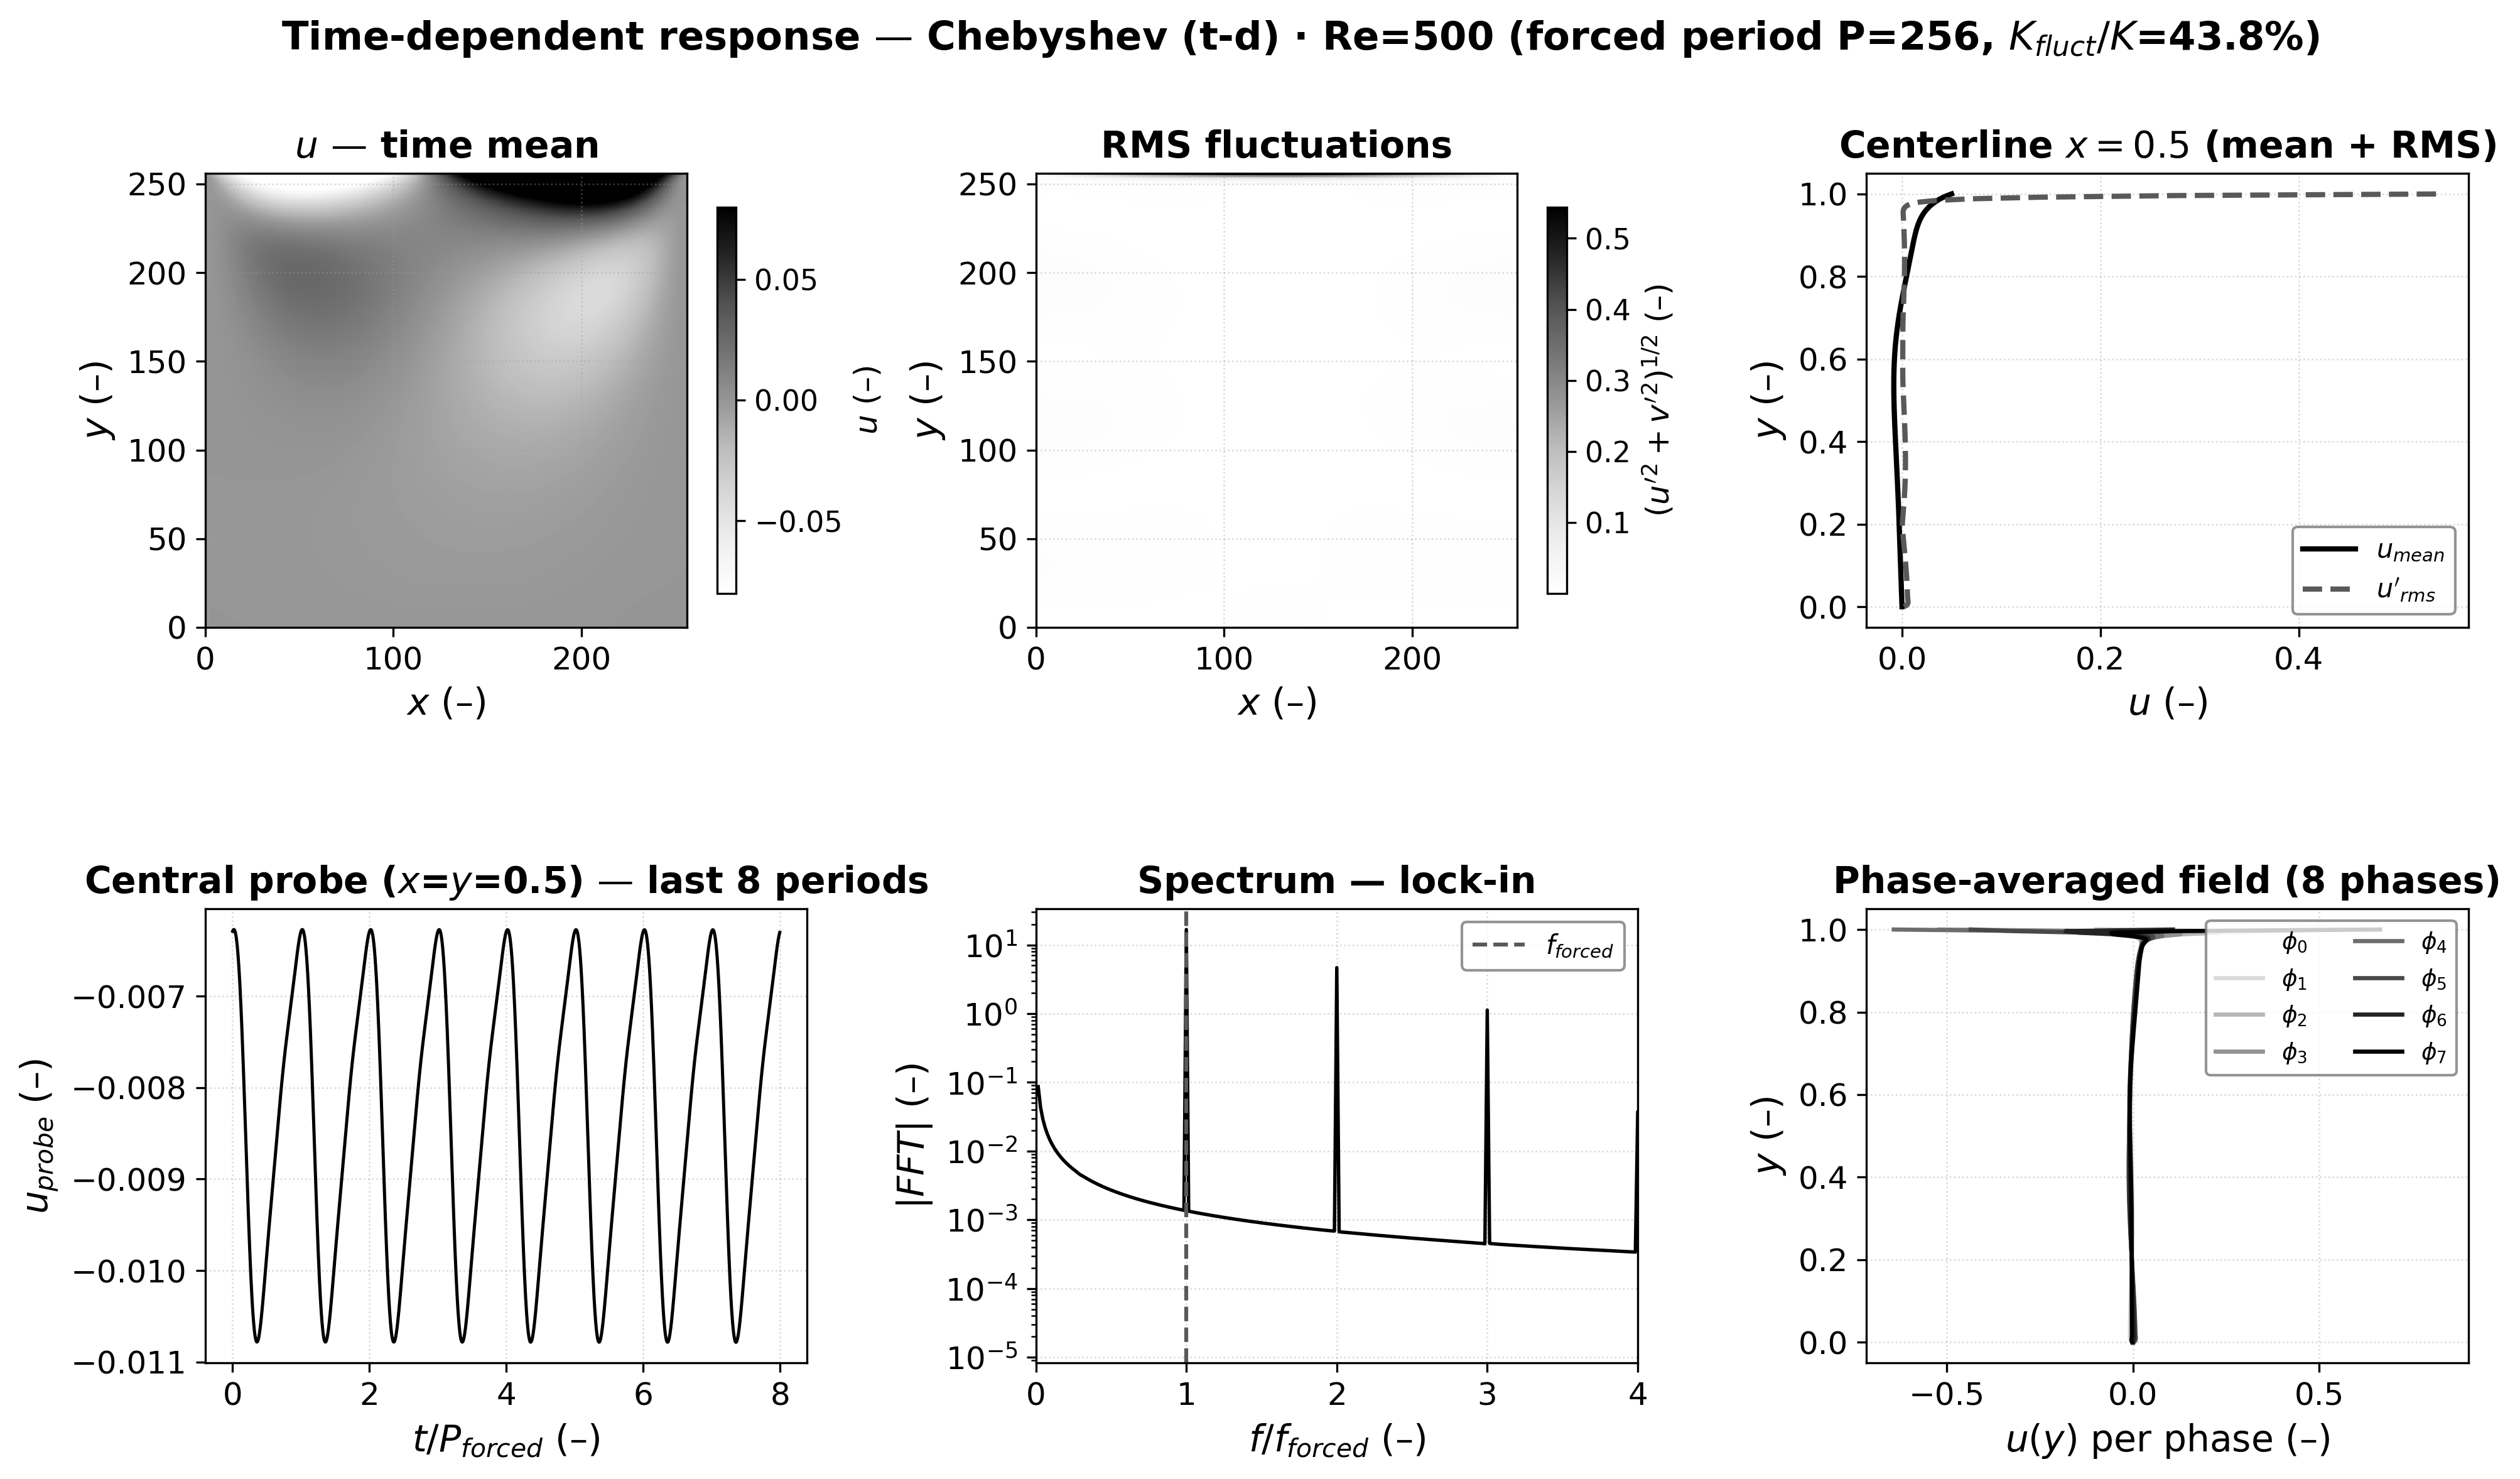
\includegraphics[width=0.8\textwidth]{figures/si_cheb_t_Re500.png}
\caption{Temporal response of the LBM realization to the time-dependent modified-Chebyshev control at $\re=500$.}
\label{fig:s12}
\end{figure}

\begin{figure}[h]
\centering
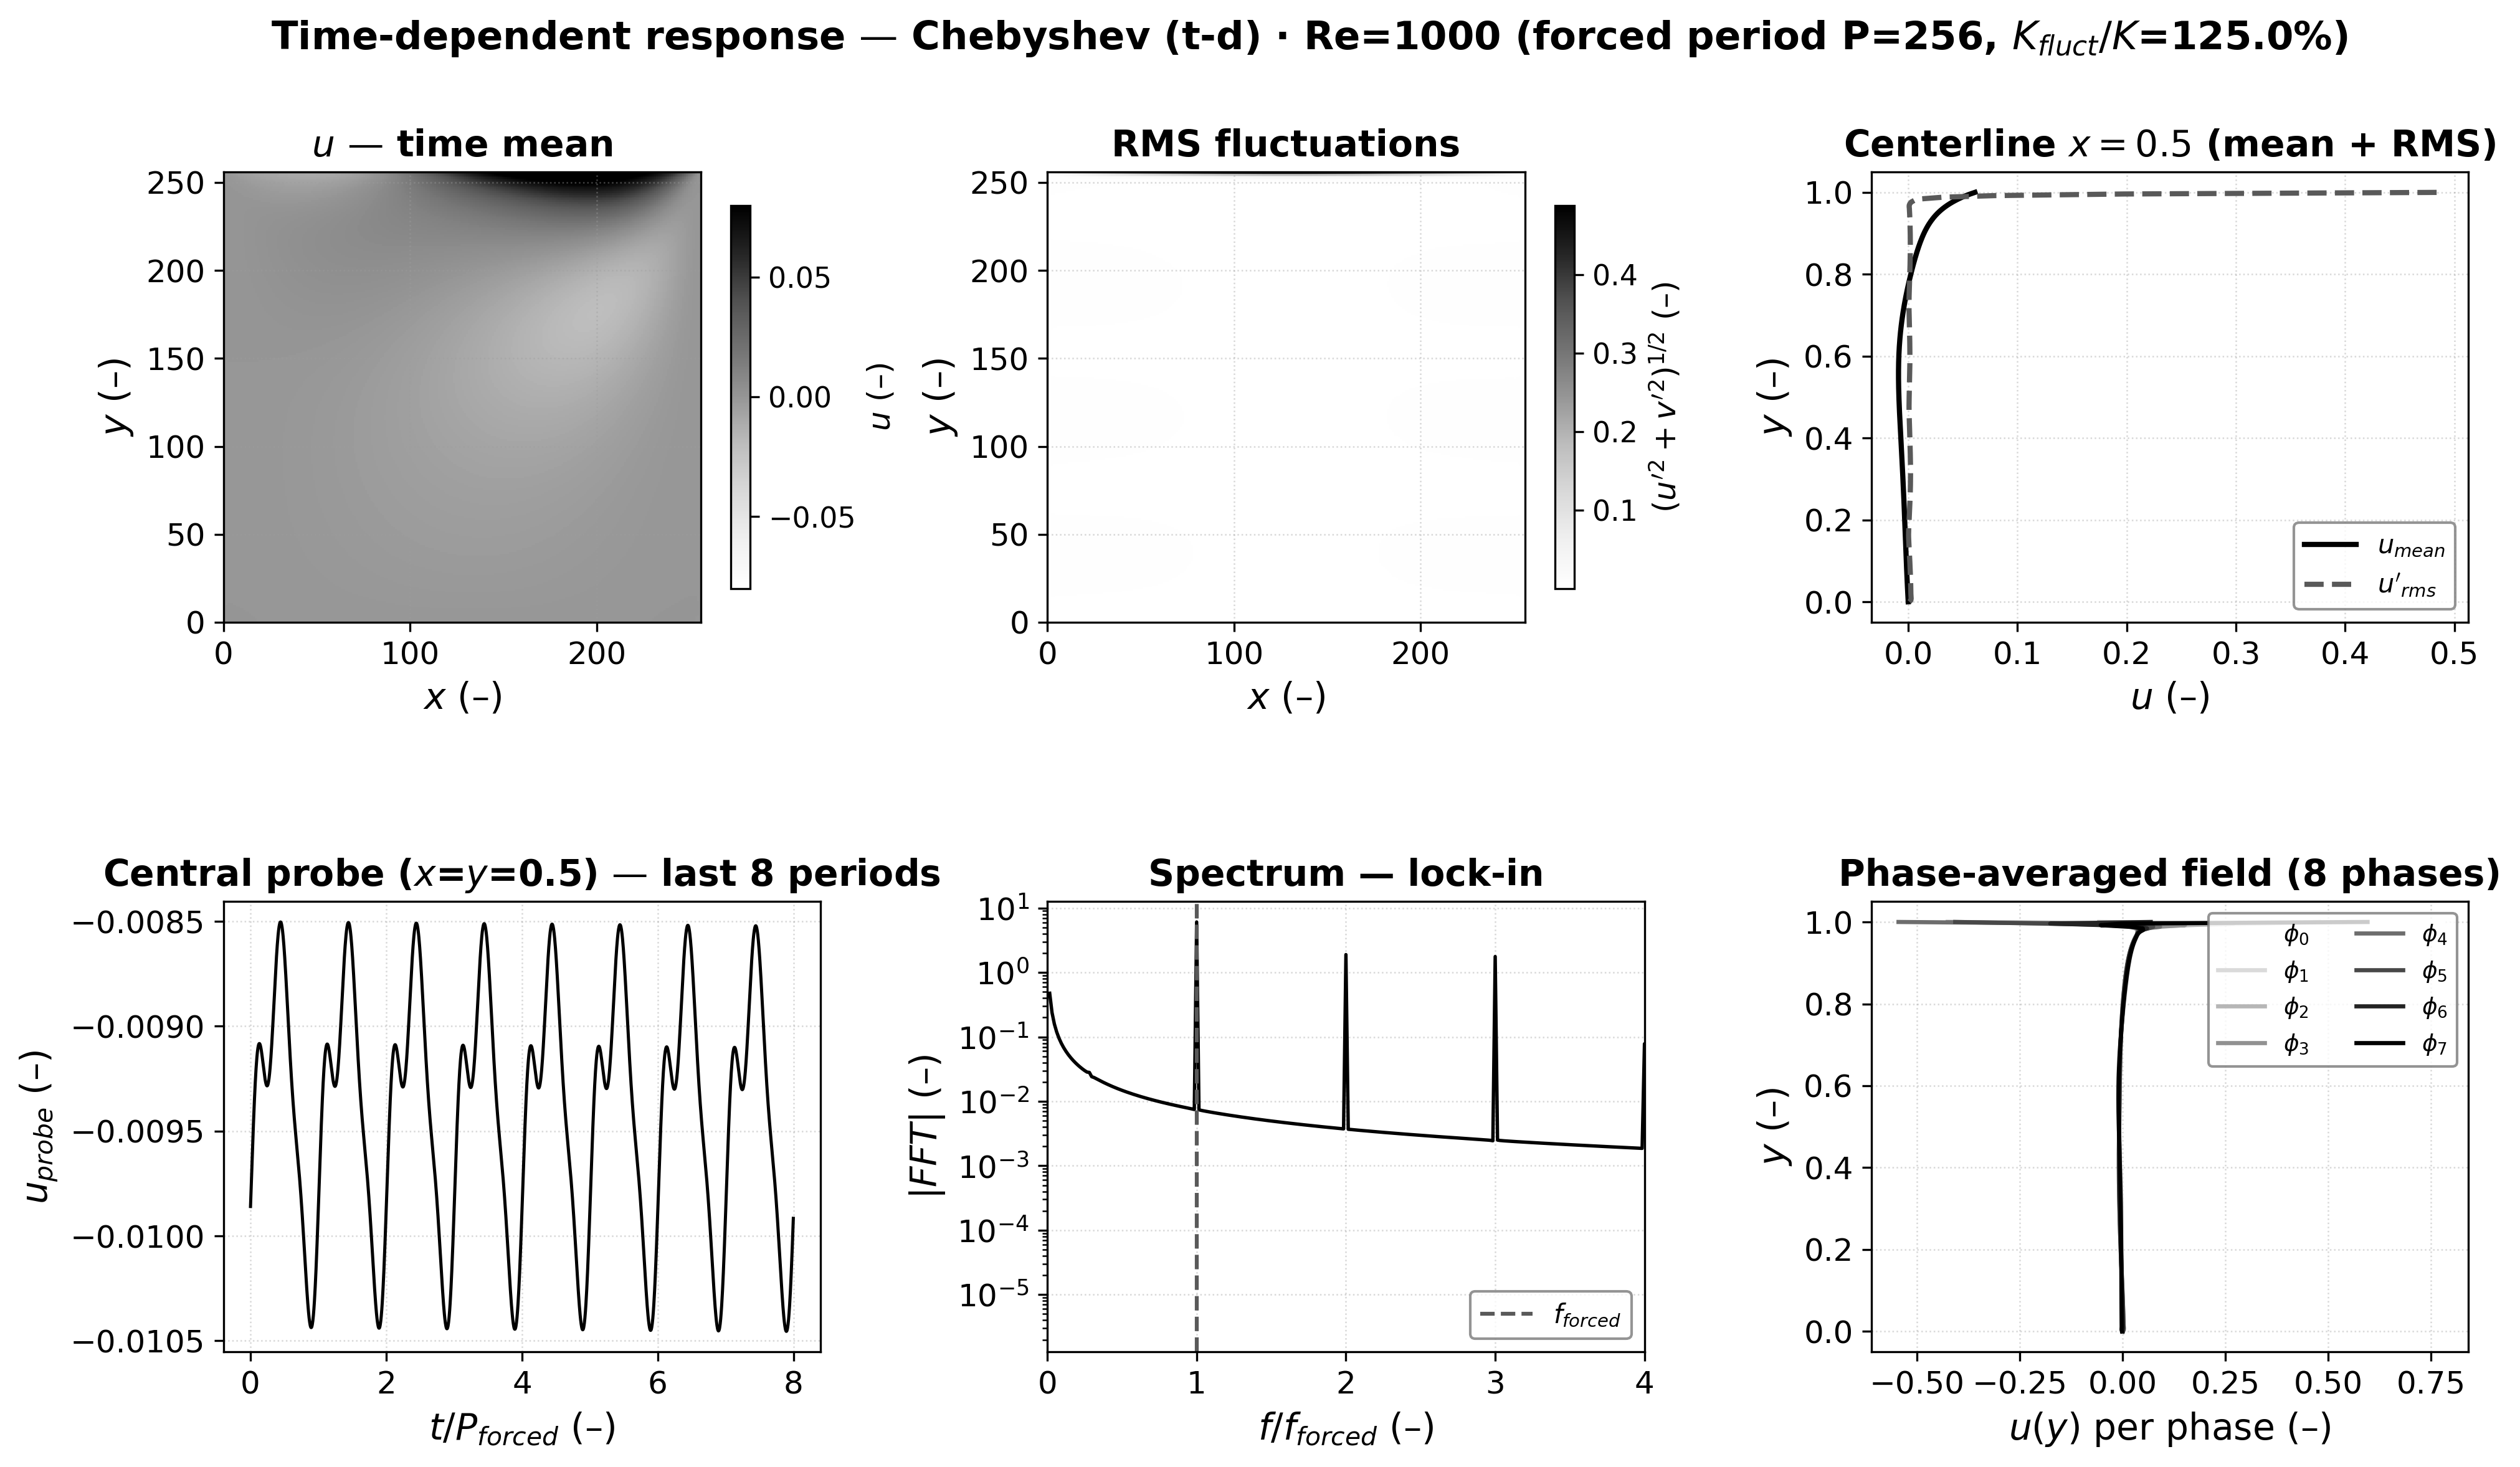
\includegraphics[width=0.8\textwidth]{figures/si_cheb_t_Re1000.png}
\caption{Temporal response of the LBM realization to the time-dependent modified-Chebyshev control at $\re=1000$.}
\label{fig:s13}
\end{figure}

\section{Temporal response of all tested controls}

Figure~S14 collects the time series and fluctuation content of the LBM realizations under all tested controls at the three Reynolds numbers, including the uniform, $\sin(\pi x)$, $A_2\sin(2\pi x)$, PINN mean, and time-dependent Fourier and modified-Chebyshev profiles. The Fourier-related profiles settle into quasi-stationary states, whereas the modified-Chebyshev profile remains strongly time-dependent.

\begin{figure}[h]
\centering
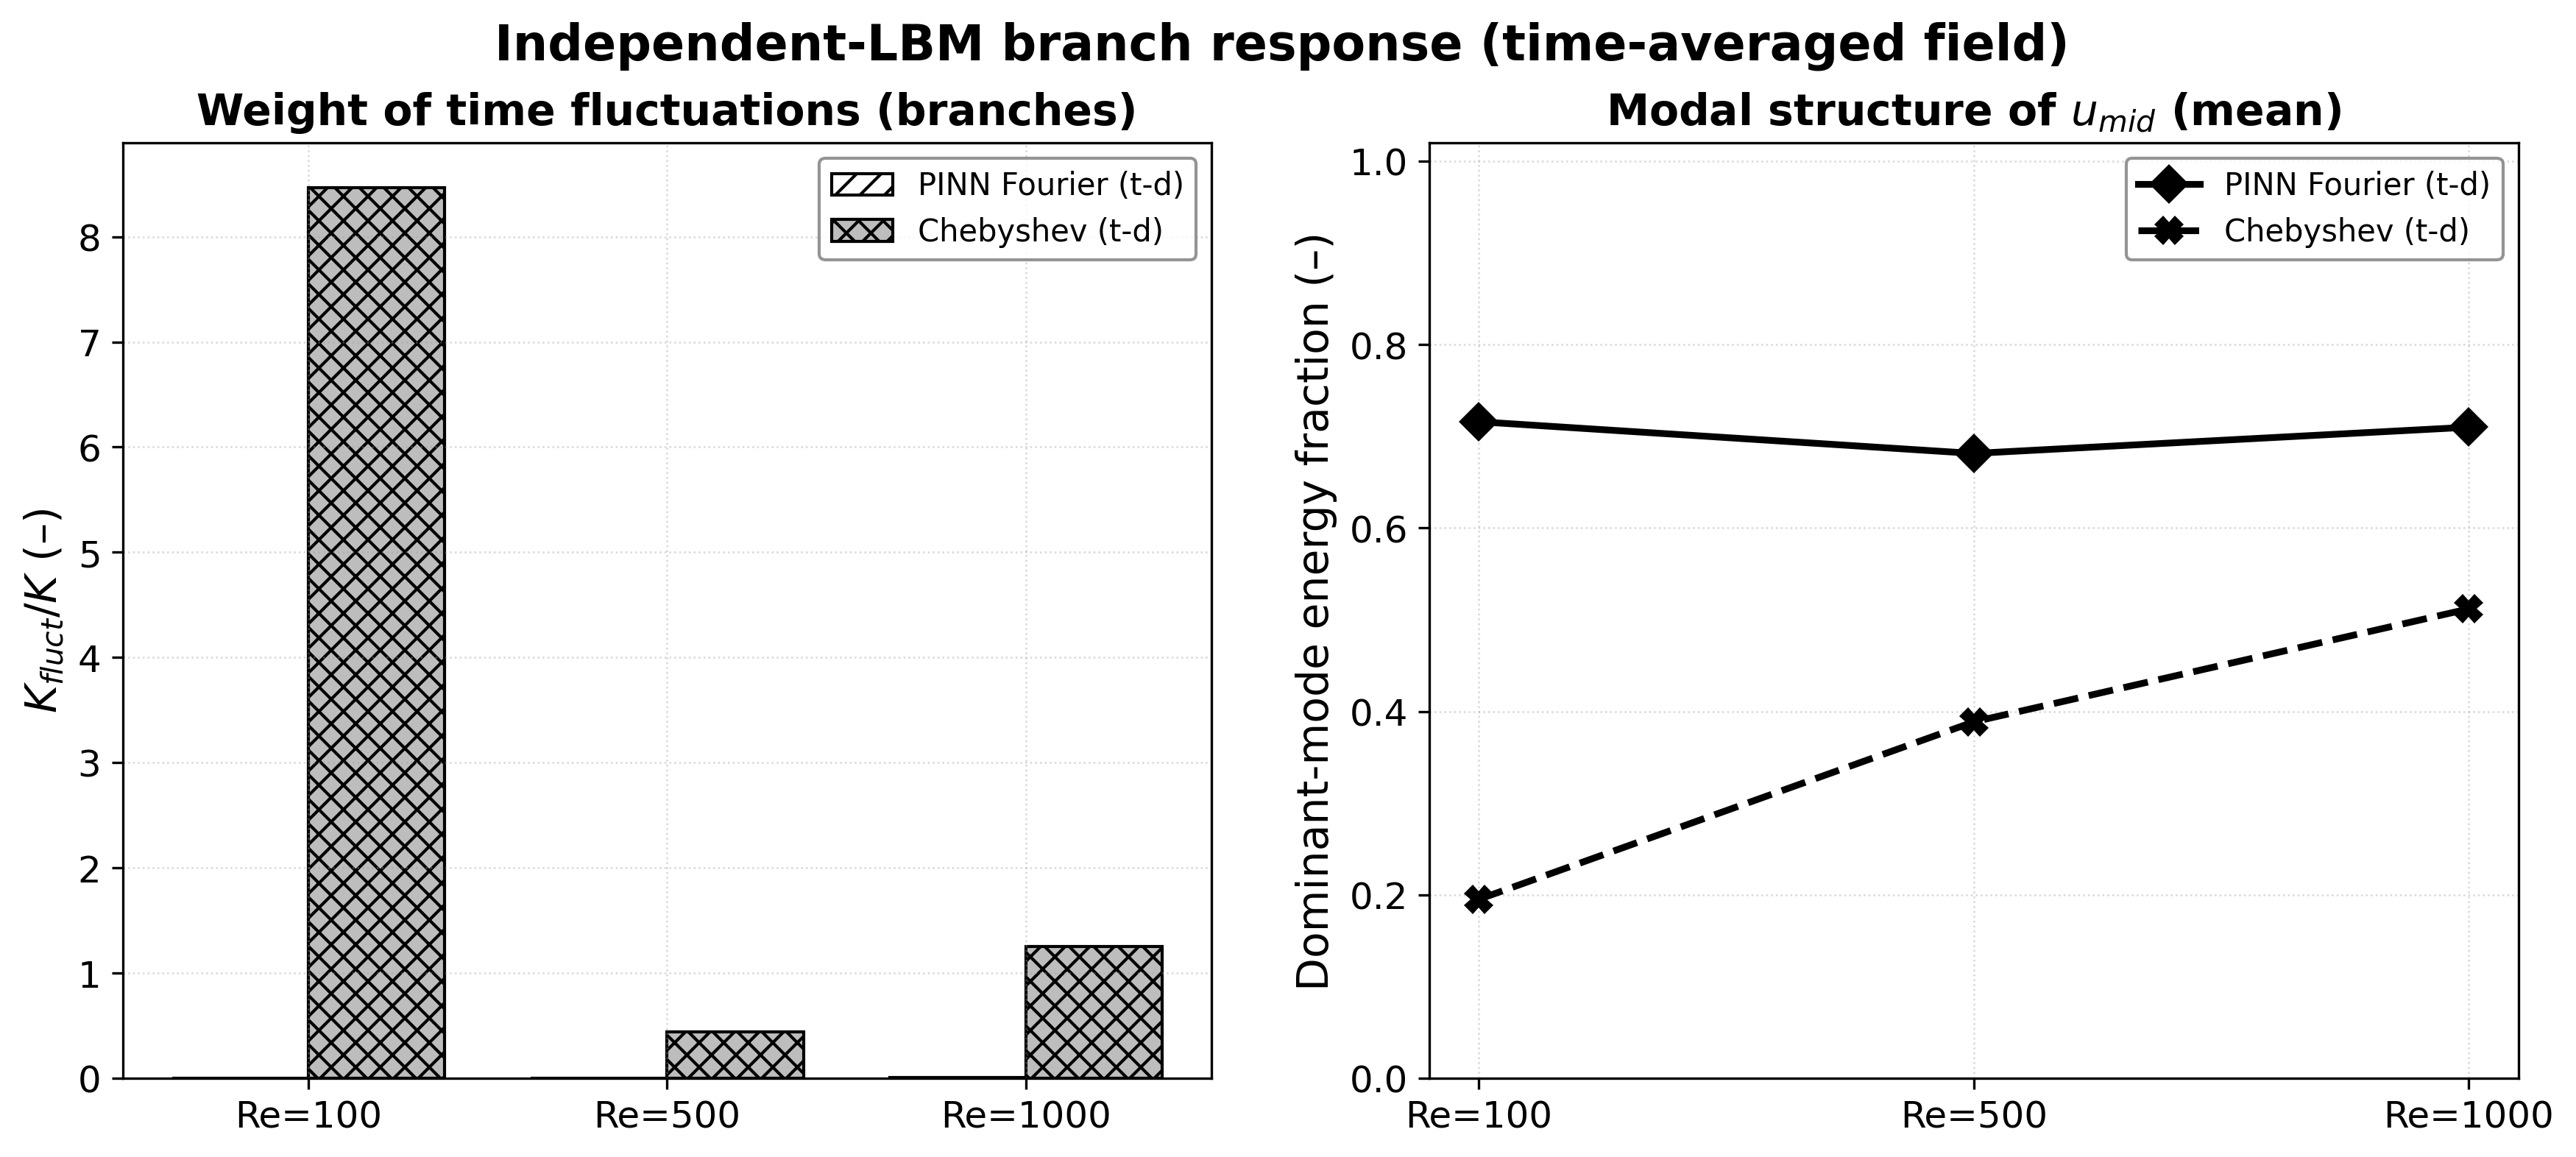
\includegraphics[width=0.8\textwidth]{figures/fig11_branches.png}
\caption{Global temporal response of the LBM realizations under all tested lid controls at $\re=100$, $500$, and $1000$. The time-dependent Fourier branch (PINN $t$-dependent) is quasi-stationary, while the modified-Chebyshev branch remains strongly time-dependent.}
\label{fig:s14}
\end{figure}

\section{Implementation and runtime notes}

All identification runs used the same software versions and the architecture, initialization, and loss weights described in the main text. The seed study repeated the training from ten independent initializations, and the architecture sweep from three. Point sampling: each epoch resamples $N_{\mathrm{PHYS}}=4000$ interior points and $N_{\mathrm{BC}}=600$ boundary points; the pre-training phase runs for 300 epochs with the control coefficients frozen, followed by the joint optimization for 3000 epochs. Computations used double precision (64 bit). A single training run takes on the order of tens of minutes on one NVIDIA GPU; the seed, energy-sweep, architecture, mode-count, and aspect-ratio campaigns were run in sequence on the same hardware. The LBM validation used a D2Q9 lattice with an MRT collision operator, a $256\times256$ production grid (grid-convergence study on $128$, $256$, and $512$ grids), a convergence tolerance of $10^{-9}$ on the integrated dissipation, and a cap of $10^6$ iterations for the Ghia validation runs.

\end{document}